\chapter{Hybrid Systems} \label{chap:HS}

%\begin{abstract}
This chapter, which is based on \citeK{Kaushik16_ICC}, studies the performance of hybrid cognitive radio systems that combine the benefits of interweave and underlay systems by employing a spectrum sensing and a power control mechanism at the Secondary Transmitter (ST). It is discussed that the existing baseline models considered for performance analysis assume perfect knowledge of the involved channels at the ST, however, analog to the interweave and the underlay scenarios investigated in chapters \ref{chap:IS} and \ref{chap:US}, such situations hardly exist in practical deployments. Motivated by this fact, a novel approach that incorporates channel estimation at the ST is proposed, which consequently characterizes the performance of Hybrid Systems (HSs) under realistic scenarios. To capture the impact of imperfect channel knowledge, outage constraints on the detection probability at the ST and on the interference power received at the primary receiver are propsed. The analysis reveals that the baseline model overestimates the performance of the HS in terms of achievable secondary user throughput. An estimation-sensing-throughput tradeoff is established to determine a suitable estimation and a sensing durations that effectively capture the effect of imperfect channel knowledge and subsequently enhance the achievable secondary user throughput. 
%\end{abstract}
%%%%%%%%%%%%%%%%%%%%%%%%%%%%%%%%%%%%%%%%%%%%%%%%%%%%%%%%%%%%%%%%%%%%%%%%%%%%%%%%%%%%%%%%%

%\section{Introduction}%%%%%%%%%%%%%%%%%%%%%%%%%%%%%%%%%%%%%%%%%%%%%%%%%%%%%%%%%%%%%%%%%%%%%%%%%%%%%%%%%%%%%%%%%
%\subsection{Background}
%Cognitive Radio (CR) communication is considered as one of the potential solutions that addresses the spectrum scarcity problem of future wireless networks. According to Goldsmith \textit{et al.} \cite{Goldsmith09}, secondary access to the licensed spectrum can be associated with different CR paradigms, which are employed by the secondary system. These paradigms include interweave, underlay and overlay systems. Since interweave and underlay systems are mainly associated with the physical layer, they are considered for hardware implementations. According to interweave systems, Secondary Users (SUs) utilize the licensed spectrum opportunistically by exploiting spectral holes in different domains such as time, frequency, space, polarization, etc, whereas in underlay systems, SUs are allowed to use the primary spectrum as long as they respect the interference constraints of the Primary Receivers (PRs). 
%On the other hand, overlay systems allow the spectral coexistence of two or more wireless networks by employing advanced transmission and coding strategies. 
%Recently, Hybrid Systems (HSs) that exploit the benefits of interweave and underlay systems for performance enhancement have been introduced. In this regard, this work focuses on performance characterization of the HSs that incorporates estimation of the involved channels.
\section{Related Work}

Underlay systems employ several techniques such as power control, interference alignment, beamforming that allow CR systems to mitigate the interference at the primary systems \cite{Sharma15}. More particularly, the underlay systems tend to operate below a certain level defined as the Interference Threshold (IT). 
In the context of an interweave system, the interference is avoided by sensing a licensed spectrum or Primary User (PU) signal at the Secondary Transmitter (ST).
Spectrum sensing can be performed by employing various techniques such as energy detection, matched filter based detection, cyclostationary based detection \cite{Sharma15}. Due to its versatility towards the unknown primary user signal, energy detection is considered for performing spectrum sensing. In this view, the performance of interweave systems depend on the detector's performance, which is characterized in terms of detection probability and false alarm probability. 
As a result, to ensure that the interference is restricted below a certain level, it is essential to operate the detector in such a way that the detection probability stays above a desired level. Besides that, the performance of the secondary system can be characterized in terms of throughput achieved at the Secondary Receiver (SR), which is generally influenced by the false alarm probability. In this context, a fundamental relationship between the sensing and the secondary throughput has been investigated by Liang \textit{et al.} \cite{Liang08}. 

However, the interweave system does not account for the severity of the interference power received at the PR, which in most cases can be tolerated by the primary systems and in other cases can lead to outage at the PR, thereby resulting in serious performance degradation of the primary system. In contrast to the interweave systems, the detection incapability of underlay systems forbids them to transmit with full power, specially during the periods when the primary system remains inactive. Addressing these issues can significantly enhance the spectral efficiency of the CR systems. In this context, a joint solution that utilizes the interference tolerance capability of the underlay systems and the agility of interweave systems to detect spectrum holes, defined as Hybrid System (HS), has been proposed \cite{Kang09, Oh10, Senthu12, Jiang13, Sharma14}. 

Kang \textit{et al.} \cite{Kang09} established a frame structure for HSs, whereby the ST first senses a PU channel in order to decide its operation mode (interweave or underlay) based on the detection result. Further, to decide upon a suitable operation mode, appropriate strategies that maximize the secondary system's throughput have been investigated by Oh \textit{et al.} \cite{Oh10} and Senthuran \textit{et al.} \cite{Senthu12}, respectively. Besides that, Jiang \textit{et al.} employed a double detection threshold, which enables dynamic switching between full and partial access modes. Lastly, a sensing-throughput tradeoff to characterize the performance of the HS has been investigated by Sharma \textit{et al.} \cite{Sharma14}. 
%The prime objective to access scheme 
Considering the fact that most of the existing models \cite{Kang09, Oh10, Senthu12, Jiang13, Sharma14} used for performance analysis assume the perfect knowledge of the involved channels at the ST. This assumption is however not viable for practical implementations, thereby rendering the performance analysis carried out using these models inaccurate. In this context, the performance analysis of the HS that incorporates channel estimation is an interesting research problem. Motivated by this fact, this chapter establishes a fundamental framework that considers the estimation of the involved channels and characterizes the impact of estimation errors on CR system performance.
\section{Contributions}
More specifically, this chapter provides the following contributions:
\begin{itemize}
\item 
A novel analytical framework for the HS that constitutes the estimation of interacting channels, namely: (i) sensing channel, (ii) interference channels and (iii) access channel is established.
\item
Based on the proposed framework, the impact of imperfect channel knowledge is investigated in terms of the interference encountered at the PR. Particularly, to restrict this interference, an outage constraints on the detection probability at the ST and on the interference power received at the PR is employed. Consequently, the performance of the HS in terms of the achievable secondary throughput is analyzed.
\item 
Finally, a fundamental tradeoff between estimation time, sensing time and achievable throughput is derived. This tradeoff is exploited to determine suitable estimation and sensing durations that achieve a maximum performance for the HS in terms of the secondary throughput. 
%Finally, the performance of the HS is characterized based on analytical expressions.
\end{itemize}
%\subsection{Organization}
%\imp{Can be done at the end.}

%The subsequent sections of the paper are organized as follows: Section \ref{sec:sys_mod} describes the system model that includes the deployment scenario, the signal model and the performance analysis based on the ideal model. Section \ref{sec:pm} presents the proposed model that incorporates channel estimation, characterization of the involved parameters and subsequently performance analysis in terms of sensing-throughput tradeoff. Section \ref{sec:num_ana} analyzes the numerical results based on the expressions obtained expressions. Finally, Section \ref{sec:conc} concludes the paper. 
%%%%%%%%%%%%%%%%%%%%%%%%%%%%%%%%%%%%%%%%%%%%%%%%%%%%%%%%%%%%%%%%%%%%%%%%%%%%%%%%%%%%%%%%%
\section{System Model} \label{sec:sys_mod}
%%%%%%%%%%%%%%%%%%%%%%%%%%%%%%%%%%%%%%%%%%%%%%%%%%%%%%%%%%%%%%%%%%%%%%%%%%%%%%%%%%%%%%%%%
\subsection{Deployment Scenario and Medium Access}
%Cognitive Small Cell (CSC), a CR application, characterizes a small cell deployment that fulfills the spectral requirements for Mobile Stations (MSs) operating indoor, cf. \figurename~\ref{fig:scenario}.
%For the disposition of the CSC in the network, the following key elements are essential: a CSC-Base Station (CSC-BS), a Macro Cell-Base Station (MC-BS) and MS \cite{Kaushik16}.
Considering the fact that the spectrum sensing and power control are employed at the CSC-BS, the CSC-BS and the MS represent ST and SR, respectively. As an extension to the existing models depicted in \cite{Kang09, Sharma14}, a slotted medium access for the HS, where the time axis is segmented into frames of length $T$ is considered, according to which, the ST employs periodic sensing. In this view, each frame consists of a sensing interval $\tsen$ followed by data transmission ($T - \tsen$). Depending on the outcome of the sensing, the data transmission takes place  with or without power control. 
\begin{figure}[!t]
\centering
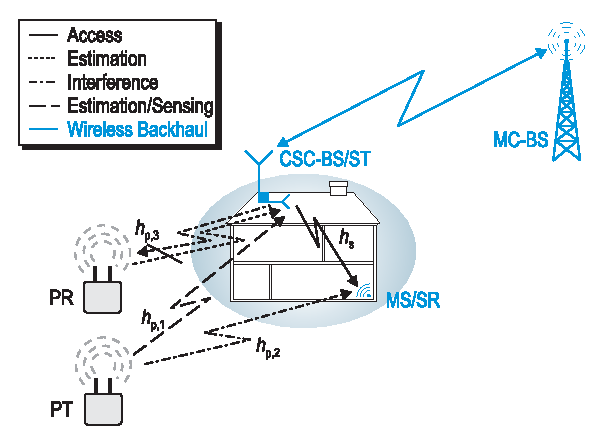
\includegraphics[width = \figscalet]{figures/CR_Scenario_Hybrid}
\caption{A cognitive small cell scenario demonstrating: (i) the underlay paradigm, (ii) the associated network elements, which constitute Cognitive Small Cell-Base Station/Secondary Transmitter (CSC-BS/ST), Mobile Station/Secondary Receiver (MS/SR), Macro Cell-Base Station (MC-BS) and Primary Transmitter (PT), (iii) the interacting channels: sensing ($\hpo$), interference ($\hptw, \hpth$) and access ($\hs$) channels.}
\label{fig:scenario}
%\vspace{-6mm}
\end{figure}
%\subsubsection{Medium access}

%The duration $T$ ($\ll$ expected ON/OFF period of the primary user) is chosen in such a way that the frames are aligned to contolled based transmissions \cite{Kaushik16, Kaushik16_CL}. The frame structure is to periodic sensing/estimation in IS \cite{Liang08}. 
%HS uses $\tau$ to estimate the received power, where $\tau (< T)$ corresponds to a time interval. To incorporate fading in the model, we assume that the channel remains constant for $T$. Hence characterized by the fading process, each frame witnesses a different received power. Therefore to sustain a desired probability of confidence, it is important to exercise estimation followed by power control for each frame. Thus, the time $T - \tau$ is utilized for data transmission with controlled power. 

%For the mentioned techniques, we consider a proper alignment of the ST to the PR transmissions. Hence, during data transmission at the ST, the SR procures no interference from the PR, cf. \figurename~\ref{fig:scenario}. 

\subsection{Signal Model}
It is considered that both primary and secondary systems employ Orthogonal Frequency Division Multiplex (OFDM) signal to carry out their transmissions. As a result, OFDM signals transmitted by the primary system are modelled as zero mean Gaussian signals by the secondary system, and vice versa. 

Subject to the underlying hypothesis, illustrating the presence $\mathcal H_1$ and the absence $\mathcal H_0$ of the primary signal, the discrete and complex received signal is given by 
\begin{equation}
\yrcvd[n] = 
\begin{cases}
\hpo \cdot \xp[n] + w[n] & : \mathcal{H}_1 \\
w[n] & :\mathcal{H}_0
\end{cases},
\label{eq:sig_mod_st}
\end{equation}
where $\xp[n]$ corresponds to a discrete and complex sample transmitted by the PT, $|\hpo|^2$ represents the power gain of the sensing channel for a given frame and $w[n]$ is circularly symmetric additive white Gaussian noise at the ST. 
The mean and variance for the signal and the noise are determined as: $\e{}{\xp[n]} = 0$, $\e{}{w[n]} = 0$, $\e{}{|\xp[n]|^2} = \spo$ and $\e{}{|w[n]|^2} = \npo$. 
The channel $\hpo$ is considered to be independent of $\xp[n]$ and $w[n]$, thus, $\yrcvd[n]$ is also an independent and identically distributed (i.i.d.) random process.

Following the conventional frame structure, ST performs periodic sensing for a duration of $\tsen$. The test statistics $\ts$ at the ST is evaluated as $\ts = \s{\tsen \fsam}{ |\yrcvd[n]|^2} \mathop{\gtrless}_{\mathcal{H}_0}^{\mathcal{H}_1} \mu$, where $\mu$ is the decision threshold and $\textbf{y}$ is a vector with $\tsen \fsam$ samples. $\ts$ represents a random variable, whereby the characterization of the distribution function depends on the underlying hypothesis. Corresponding to the considered PU signal model, $\ts$ follows a central chi-squared ($\cchi2$) distribution for both hypotheses $\mathcal H_0$ and $\mathcal H_1$ \cite{Kay}.
Consequently, the detection probability $(\pd)$ and the false alarm probability $(\pfa)$ are determined as \cite{Tan08}
\begin{align}
\pd(\mu, \tsen, \prcvdstpt) &= \Gamma\left( \frac{\tsen \fsam}{2}, \frac{\tsen \fsam \mu}{2 \prcvdstpt} \right),  \label{eq:pd} 
\end{align}
\begin{align}
\pfa(\mu, \tsen) &= \Gamma\left( \frac{\tsen \fsam}{2}, \frac{\tsen \fsam \mu}{2 \npo} \right),  \label{eq:pfa} 
\end{align}
where $\prcvdstpt$ is the power received over the sensing channel and $\Gamma(\cdot, \cdot)$ represents a regularized upper incomplete Gamma function \cite{grad}.

Similar to (\ref{eq:sig_mod_st}), the discrete and complex received signal at the SR conditioned on the sensing outcome is given by 
\begin{equation}
\hspace{-2.3mm}
\ys[n] = 
\begin{cases}
\hs \cdot \xsfull[n] + \hptw \cdot \xp[n] + w[n] &: 1 - \pd \\
\hs \cdot \xsfull[n] + w[n] &: 1 - \pfa \\
\hs \cdot \xscont[n] + \hptw \cdot \xp[n] + w[n] &: \pd \\
\hs \cdot \xscont[n] + w[n] &: \pfa 
\end{cases},
\label{eq:sig_mod_sr}
\end{equation}
where $\xsfull[n]$ and $\xscont[n]$ present the discrete and complex samples with full transmit power $\pfull$ and controlled transmit power $\preg$, respectively. Additionally, $|\hs|^2$ and $|\hptw|^2$ represent the power gains for the access and the interference channels, cf. \figurename~\ref{fig:scenario}. 


Besides that, an interference from the ST is encountered at the PR across the channel $\hpth$ only for the cases where the PT is transmitting, i.e., $(1 - \pd, \pd)$, cf. (\ref{eq:sig_mod_sr}). In this regard, the interference signal from the ST at the PR is given by
\begin{equation}
\yp[n] = 
\begin{cases}
\hpth \cdot \xscont[n] + w[n] & : \pd \\
\hpth \cdot \xsfull[n] + w[n] & : 1- \pd 
\end{cases}.
\label{eq:sig_mod_pr}
\end{equation}

\subsection{Problem Description}
To employ a power control mechanism, the ST is required to control its transmit power in such a way that the interference power received at the PR is below a certain interference threshold ($\ite$). In reference to the HS, constraints on interference power received at the PR are defined as
\begin{align}
\pho \cdot \pd \cdot \phpth \preg \le \ite \label{eq:IT_ida} \\
\intertext{and   } 
\pho \cdot (1 - \pd) \cdot \phpth \pfull \le \ite \label{eq:IT_idb},
\end{align}
where $\pho$ $(= 1 - \phz)$ represents the occurrence probability of the hypothesis $\mathcal H_1$. 
According to \cite{Sharma14}, (\ref{eq:IT_idb}) is usually handled by the regulatory bodies. In this regard, using (\ref{eq:IT_ida}) and the knowledge of $\ite$, the controlled power is computed as $\frac{\ite}{\pho \cdot \pd \cdot \phpth}$.

Next, the throughput received at the SR corresponding to the cases illustrated in (\ref{eq:sig_mod_sr}) is characterized. Subject to the sensing outcome $1 - \pfa, 1 - \pd, \pfa, \pd$, the corresponding throughputs at the SR are defined as 
\begin{align}
\rsz(\tsen) =& \frac{T- \tsen}{T} \cdot \smash[b]{\overbrace{\log_2 \left(1 + |\hs|^2 \frac{\pfull}{\npo}\right)}^{\cz}} \nonumber \\ 
\quad & \times (1 - \pfa ) \cdot \phz,  \label{eq:Cap0} \\ 
\rso(\tsen) =& \frac{T- \tsen}{T} \smash[b]{\overbrace{\log_2 \left(1 + \frac{|\hs|^2 \pfull }{|\hptw|^2 \ptranpt  + \npo} \right)}^{\co}} \nonumber \\ 
\quad & \times (1 - \pd) \cdot \pho,  \label{eq:Cap1} \\ 
\rstw(\tsen) =& \frac{T- \tsen}{T} \cdot \smash[b]{\overbrace{\log_2 \left(1 + |\hs|^2 \frac{\preg}{\npo}\right)}^{\ctw}} \nonumber \\ 
\quad & \times \pfa \cdot \phz,  \label{eq:Cap2} \\ 
\rsth(\tsen) =& \frac{T- \tsen}{T} \cdot \smash[b]{\overbrace{\log_2 \left(1 + \frac{|\hs|^2 \preg }{|\hptw|^2 \ptranpt  + \npo} \right)}^{\cth}}  \nonumber \\   
\quad & \times \pd \cdot \pho.  \label{eq:Cap3}  
%\text{where  } & \preg = \frac{\ptranpr \cdot \ite}{|\hpth|^2}.
\end{align}
%where ${|\hptw|^2 \ptranpt  + \npo}$ in (\ref{eq:Cap1}) and (\ref{eq:Cap3}) represents the interference power received from the PT.
where $\cz, \co, \ctw$ and $\cth$ represent the data rates.

Sharma \textit{et. al.} \cite{Sharma14} established a tradeoff between the sensing time and secondary throughput $(\rs)$ subject to a target detection probability $(\pdd)$. This tradeoff is represented as
\begin{align}
\rs(\ttsen) &= \maxi_{\tsen} \rs(\tsen) \label{eq:opT_id}\\ 
\quad &= \rsz(\tsen) + \rso(\tsen) + \rstw(\tsen) + \rsth(\tsen) \nonumber  \\
\text{s.t.} & \text{ } \pd \ge \pdd, \label{eq:pdc_id} \\ 
\text{s.t.} & \text{ } (\ref{eq:IT_idb}). \nonumber
\end{align}
%where $\rs(\ttsen)$ corresponds to achievable secondary throughput at $\ttsen$.
As a consequence, the tradeoff depicted in (\ref{eq:opT_id}) determines a suitable sensing time $\ttsen$ that achieves the maximum secondary throughput.
However, the system model depicted above has the following fundamental issues:
\begin{itemize}
\item Without the knowledge of the received power (sensing channel, $\hpo$), the characterization of $\pd$ is not possible, cf. (\ref{eq:pd}). This leaves the constraint defined in (\ref{eq:pdc_id}) inappropriate. 
\item Without the knowledge of the interference channel towards the PR ($\hpth$), the power control mechanism cannot be employed at the ST.
\item Along with the above mentioned channels, the knowledge of the access ($\hs$) and interference channel ($\hptw$) to the SR, from the PT, is required at the ST for characterizing the secondary throughput. 
\end{itemize} 
With these issues, it is not reasonable to consider the performance analysis depicted by the ideal model (described as baseline models) for hardware implementation. In order to address these issues, an analytical framework that includes the estimation of these channels and characterizes the performance of the HS in terms of the sensing-throughput tradeoff is proposed. 
%%%%%%%%%%%%%%%%%%%%%%%%%%%%%%%%%%%%%%%%%%%%%%%%%%%%%%%%%%%%%%%%%%%%%%%%%%%%%%%%%%%%%%%%%
\section{Proposed Approach} \label{sec:pm}
%%%%%%%%%%%%%%%%%%%%%%%%%%%%%%%%%%%%%%%%%%%%%%%%%%%%%%%%%%%%%%%%%%%%%%%%%%%%%%%%%%%%%%%%%
\subsection{Frame Structure}
\begin{figure}[!t]
\centering
%\subfloat[]{
%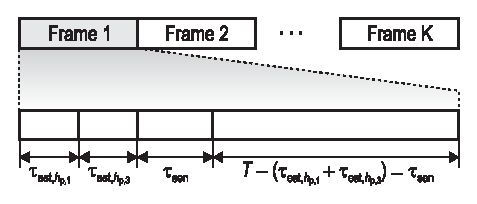
\includegraphics[width = \figscalet]{figures/Frame_Structure_grau}
%} \\
%\subfloat[]{
\includegraphics[width = \figscalett]{figures/Frame_Structure}
%}
\caption{Frame structure of HSs illustrating the time allocation for channel estimation, sensing and data transmission from the perspective of a ST and a SR.} 
\label{fig:fs}
%\vspace{-7mm}
\end{figure}
In order to incorporate the estimation of the involved channels, a novel frame structure is proposed in \figurename~\ref{fig:fs}, according to which, $\testpt$ and $\testptsr$ are utilized for estimating $\hpo$ and $\hptw$ by the ST and SR\footnote{In order to accomplish this, it is assumed that both the ST and the SR align themselves to the control-based transmission from the PT.}, respectively. Besides that, $\testpr$ is used for estimating the $\hpth$. Since the ST considers the estimation based on the pilot symbols transmitted by the ST that already exist in the secondary system, no time resources are allocated for the estimation of $\hs$. However, it is possible that the time interval between two control-based transmissions is large as compared to $T$. Under such conditions, the frame structure followed by the secondary system can be adapted from the one proposed in \figurename~\ref{fig:fs} in such a way that channel estimation is restricted to particular frames and the remaining frames follow the conventional structure, i.e., sensing followed by data transmission. Hence, the proposed frame structure presents a general framework and is adaptable to different control-based configurations followed by various primary systems. For scenarios, where the PT and the PR represent a single entity, i.e., interchangeably act as transmitter and receiver, the first two slots $\testpt$ and $\testpr$ of the ST can be combined into one, cf. \figurename\ref{fig:fs}. 


\subsection{Channel Estimation}
Here, the estimation of the interacting channels is revisited. In this chapter, a similar approach for the channel estimation to the one described in chapters \ref{chap:IS} and \ref{chap:US}, according to which, it is logical to employ a received power-based estimation for the sensing and the interference channels, and a pilot-based estimation for the access channel.  
\subsubsection*{Sensing Channel ($\hpo$)}
The ST estimates the sensing channel by estimating the received power from the PT during $\testpt$. With $\testpt \fsam$ samples used for estimation, the estimated received power $\eprcvdstpt = \sum_{n = 1}^{\testpt \fsam} |\hpo \xp[n] + w[n]|^2$ follows a $\cchi2$ distribution.
%\begin{lemma} \label{lm:lm1}
The cumulative distribution function (CDF) of $\eprcvdstpt$ is characterized as
\begin{align}
\feprcvdstpt(x) = 1 - \Gamma \left( \frac{\testpt \fsam}{2}, \frac{\testpt \fsam x}{2 \prcvdstpt} \right) \label{eq:fprcvdstpt}.
\end{align}
%\end{lemma}
In order to improve the detector's performance, the samples $\fsam \testpt$ considered for the estimation can also be utilized for the sensing $\fsam \tsen$ as illustarted in \figurename~\ref{fig:fs}. In this sense, hereafter, the characterization of the detector incurs the time interval $\testpt$. 
  
\subsubsection*{Access Channel ($\hs$)}
The pilot signal received from the SR undergoes matched filtering and demodulation at the ST, hence, a pilot-based estimation at the ST is employed to acquire the knowledge of the access channel. The maximum-likelihood estimate of $\ehs$ presented by \cite{Gifford08} is unbiased, efficient, i.e., achieves a Cram\'er-Rao bound with equality and asymptotic variance $\e{}{|\hs -\ehs|^2} = \frac{\npo}{2 \Ks}$, where $\Ks$ denotes the number of pilot symbols. As a result, $\ehs$ conditioned on $\hs$ follows a Gaussian distribution
%\begin{align*}
$\ehs|\hs \sim \mathcal{N}\left( \hs,\frac{\npo}{2 \Ks} \right)$.
%\label{eq:ehs} 
%\end{align*}
Consequently, the estimated power gain $|\ehs|^2$ follows a non-central chi-squared $\ncchi2(\ls, 1)$ distribution with 1 degree of freedom and non-centrality parameter $\ls = \frac{2 \Ks \phs}{\npo}$. For analytical tractability the following approximation is considered. 
\begin{approxi} \label{ap:ap1}
\normalfont 
For all degrees of freedom, the $\ncchi2$ distribution can be approximated by a Gamma distribution \cite{abramo}. The parameters of the Gamma distribution are obtained by matching the first two central moments to those of $\ncchi2$.
\end{approxi}
%\begin{lemma} \label{lm:lm2}
Following Approximation \ref{ap:ap1}, the CDF of $\ephs$ is characterized as
\begin{align}
\fephs(x) \approx 1 - \Gamma \left(a, \frac{x}{b} \right) \label{eq:fephs}, 
\end{align}
\begin{align}
\text{where  } a = \frac{(1 + \ls)^2}{2 + 4 \ls} &\text{ and } b = \frac{\nps (2 + 4 \ls)}{(1 + \ls)}.  \label{eq:para_hs} 
\end{align}
%\end{lemma}

\subsubsection*{Interference Channel ($\hptw$)}
Besides the access channel, the knowledge of the interference channel to the SR from the PT is required for determining the secondary throughput. It is worthy to note that the expression $\phptw \spo + \npo$ in $\rso$ and $\rsth$, cf. (\ref{eq:Cap1}) and (\ref{eq:Cap3}), which corresponds to the interference and the noise power, represents $\prcvdsr$. Hence, by estimating $\eprcvdsr$, it is possible to jointly characterize the interference and the noise, and consequently characterize $\rso$ and $\rsth$.  
In this view, the SR estimates received power by listening to the control-based transmission from the PT, cf. \figurename~\ref{fig:fs}. Similar to the sensing channel, the CDF of the estimated interference power received $\eprcvdsr$ at the ST is characterized as
\begin{align}
\feprcvdsr(x) = 1 - \Gamma \left( \frac{\testptsr \fsam}{2}, \frac{\testptsr \fsam x}{2 \prcvdsr} \right) \label{eq:fprcvdsr}.
\end{align}

  

\subsubsection*{Interference Channel ($\hpth$)}
Lastly, the estimation of the interference channel between the ST and the PR is essential for employing power control at the ST. Like the sensing channel, the ST estimates $\phpth$ by listening to the control-transmission from the PR. The received power estimated ($\prcvdstpr$) from $\testpr \fsam$ samples follows $\cchi2$ distribution and its CDF is given by  
\begin{align}
\feprcvdstpr(x) = 1 - \Gamma \left( \frac{\testpr \fsam}{2}, \frac{\testpr \fsam x}{2 \prcvdstpr} \right) \label{eq:fprcvdstpr}.
\end{align}

\subsection{Characterization of performance parameters}
It is clear that the estimation of the involved channels translates to the variations in the performance parameters, which include detection probability $\epd$ at the ST, power received $\eprcvdpr$ at the PR (which includes the interference and noise power) and secondary throughput $\ers$ at the SR. In particular, the variations in $\epd$ and $\eprcvdpr$ may cause severe interference to the primary system, hence, seriously degrade the performance of CR systems. This renders the existing constraints defined by the ideal model inaccurate. 
Motivated by this fact, these variations are captured by proposing new outage constraints $\opdc$ and $\opc$ on the $\epd$ and $\eprcvdpr$, respectively, as PU constraints for the HS. These constraints are defined as  
\begin{align}
\p(\epd \le \pdd) &\le \opdc \label{eq:oc_pd}, \\
\p(\eprcvdpr \ge \ite) &\le \opc \label{eq:oc_it}.
\end{align}   
In contrast to the ideal model, in the current context, it is reasonable to consider an outage over the two constraints, cf. (\ref{eq:IT_ida}) and (\ref{eq:IT_idb}), jointly in terms of the aggregate interference power received at the PR, $\eprcvdpr$. In this regard, (\ref{eq:oc_it}) is written as 
\begin{align}
%\hspace{-2mm}
& \mathbb{E}_{\epd} \Bigg[ \p \Bigg( \pho \cdot \smash[b]{\overbrace{\left( \frac{\eprcvdstpr - \npo}{\spo} \right)}^{\phpth}} \nonumber \\ & \times ((1 - \epd) \pfull + \epd \preg) \ge \ite \Bigg) \Bigg] &\le \opc \label{eq:oc_it_def}, 
\end{align}
%\begin{align}
%\e{\eprcvd}{\rs(\tsen)} = \e{}{\rsz(\tsen)} + \e{}{\rso(\tsen)} + \e{}{\rstw(\tsen)} + \e{}{\rsth(\tsen)}
%\end{align}   
where $\e{\epd}{\cdot}$ and $\p(\cdot)$ (that represents the CDF of $\eprcvdpr$) jointly capture the variations due to $\epd$ and $\eprcvdpr$. 
To proceed further, the CDF of $\epd$, $\eprcvdpr$ and $\ers$ are characterized. This is done by transforming the CDFs of the estimated parameters, characterized previously in (\ref{eq:fprcvdstpt}), (\ref{eq:fephs}), (\ref{eq:fprcvdsr}) and (\ref{eq:fprcvdstpr}). To begin with, the CDF of the $\epd$ is evaluated to characterize the constraint on the detection probability defined in (\ref{eq:oc_pd}). 
\begin{lemma} \label{lm:lem1}
\normalfont
The CDF of $\pd$ is characterized as (see chapter for proof \ref{chap:IS}) 
\begin{align}
\fpd(x) = 1 - \Gamma \left(\frac{\testpt \fsam}{2}, \frac{\testpt \fsam \tsen \fsam \mu}{4 \prcvdstpt \Gamma^{-1}(\frac{\tsen}{2}, x) } \right), 
\label{eq:fpd}
\end{align}
where $\Gamma^{-1}(\cdot, \cdot)$ is inverse function of regularized upper incomplete Gamma function \cite{grad}.
%Using (\ref{eq:fpd}), the probability density function (pdf) of $\pd$ is characterized as
%\begin{align}
%\dpd(x) = 1 - \Gamma \left(\frac{\testpt \fsam}{2}, \frac{\testpt \fsam \tsen \fsam \mu}{4 \prcvdstpt \Gamma^{-1}(\frac{\tsen}{2}, x) } \right). 
%\label{eq:dpd}
%\end{align}
\end{lemma}
Along with $\fpd$ defined in (\ref{eq:fpd}), the CDF of the $\prcvdpr$ is characterized in order to characterize the outage constraint defined in (\ref{eq:oc_it}). 
\begin{lemma} \label{lm:lem2}
\normalfont
The CDF of $\eprcvdpr$ is characterized as 
%\begin{figure*}
\begin{align}
&\fprcvdpr (x) = \nonumber \\ 
&\int\limits_0^1 \Gamma \Bigg(\frac{\testpr \fsam}{2} , \Bigg( \frac{x \spo}{\hpo \cdot ((1 - \pd) \pfull + \pd \preg)} + \npo  \Bigg) \times \nonumber \\ 
&\frac{\testpr \fsam}{2 \prcvdstpr}  \Bigg) d\fpd. 
\label{eq:fprcvdpr}
\end{align}
%\hrulefill
% The spacer can be tweaked to stop underfull vboxes.
%\vspace{-4mm}
%\end{figure*}
\end{lemma}

Besides that, since the variations in $\epd, \eprcvdstpt, \ephs$ and $\eprcvdstpr$ translate to the variations in $\ers$, these variations are captured in terms of the expected secondary throughput. More specifically, the variations in $\eprcvdstpt, \ephs$ and $\eprcvdstpr$ result in variations in capacities $\ecz, \eco, \ectw$ and $\ecth$, cf. (\ref{eq:Cap0}), (\ref{eq:Cap1}), (\ref{eq:Cap2}) and (\ref{eq:Cap3}). In this view, we characterize the probability density functions (pdfs) for $\ecz, \eco, \ectw$ and $\ecth$ in the following Lemmas.
\begin{lemma} \label{lm:lem3}
\normalfont
The pdf of $\ecz$ is defined as (refer to chapter \ref{chap:IS}) 
\begin{align}
\dcz(x) &= 2^x \ln 2 \frac{(2^x - 1)^{a_1 - 1}}{\Gamma(a_1) b^{a_1}} \exp\left(-\frac{2^x - 1}{b_1}\right),  \label{eq:den_C0}
\end{align}
%\vspace{-4mm}
\begin{align}
\text{where  } a_0 = a &\text{ and } b_0 = \frac{\pfull}{\npo} b,  \label{eq:den_C0_para} 
\end{align}
where $a$ and $b$ are defined in (\ref{eq:para_hs}).
\end{lemma}

\begin{lemma} \label{lm:lem4} 
\normalfont
The pdf of $\eco$ is defined as (refer to chapter \ref{chap:IS})  
\begin{align}
%\hspace{-2mm}
\dco(x) &= 2^x \ln 2 \frac{(2^x - 1)^{a_0 - 1} \Gamma(a_0 + a_1)}{\Gamma(a_0) \Gamma(a_1) b_0^{a_0} b_1^{a_1}} \left(\frac{1}{b_1} + \frac{2^x - 1}{b_0}\right), \label{eq:den_C1}
\end{align}
%\vspace{-4mm}
\begin{align}
\text{where  } a_1 = \frac{\Kp}{2}  \text{  and  } b_1 = \frac{2 \prcvdsr}{\npo \Kp}, \label{eq:den_C1_para} 
\end{align}
and $a_0$, $b_0$ are defined in (\ref{eq:den_C0_para}).
\end{lemma}
Following the characterization of the pdfs for $\cz$ and $\co$, the pdfs for $\ctw$ and $\cth$ can be obtained by substituting $\preg$ for $\pfull$ in (\ref{eq:den_C0}) and (\ref{eq:den_C1}).
\begin{lemma} \label{lm:lem5}
\normalfont
The pdf of $\ectw$ is defined as
\begin{align}
\dctw(x) &= 2^x \ln 2 \frac{(2^x - 1)^{a_2 - 1}}{\Gamma(a_2) b^{a_2}} \exp\left(-\frac{2^x - 1}{b_2}\right),  \label{eq:den_C2}
\end{align}
%\vspace{-4mm}
\begin{align}
\text{where  } a_2 = \frac{(1 + \ls)^2}{2 + 4 \ls} &\text{ and } b_2 = \frac{\preg}{\npo}\frac{\nps (2 + 4 \ls)}{(1 + \ls)}.  \label{eq:den_C2_para} 
\end{align}
\end{lemma}

\begin{lemma} \label{lm:lem6}
\normalfont
The pdf of $\ecth$ is defined as 
\begin{align}
%\hspace{-2mm}
\dcth(x) &= 2^x \ln 2 \frac{(2^x - 1)^{a_2 - 1} \Gamma(a_2 + a_1)}{\Gamma(a_2) \Gamma(a_1) b_2^{a_2} b_1^{a_1}} \left(\frac{1}{b_1} + \frac{2^x - 1}{b_2}\right), \label{eq:den_C3}
\end{align}
where $a_1$, $b_1$ and $a_2, b_2$ are defined in (\ref{eq:den_C1_para}) and (\ref{eq:den_C2_para}), respectively.
\end{lemma}
Subsequently, the variations arising due to $\epd$ are captured by considering $\fpd$ characterized in Lemma \ref{lm:lem1}. As a result, the expected throughput is given by (\ref{eq:exp_thr}), where $\e{\Omega}{\cdot}$ denotes the expectation over $\Omega$, where $\Omega \in \{ \epd, \ecz, \eco, \ectw, \ecth \}$ 
%\begin{figure*}
\begin{align}
&\e{\Omega}{\rs(\tsen)} = \frac{T - \testpr - \tsen}{T} \times \nonumber \\ 
&\Bigg[ (1 - \pfa) \cdot \phz \cdot \e{\ecz}{\ecz} +  (1 - \e{\epd}\epd) \cdot \pho \cdot \e{\eco}{\eco} \nonumber \\ &+  \pfa \cdot \phz \cdot \e{\ectw}{\ectw} +  \e{\epd}{\epd} \cdot \pho \cdot \e{\ecth}{\ecth} \Bigg]. \label{eq:exp_thr} 
\end{align}
The random variables $\epd$ and  $\eco, \ecth$ are functions of independent random variables $\eprcvd$ and, $\ephs$ and $\eprcvdsr$, respectively. In this context, the independence property is applied to carry out the expectation on $\epd$, $\eco$ and $\ecth$ in (\ref{eq:exp_thr}) individually.
%\hrulefill
% The spacer can be tweaked to stop underfull vboxes.
%\vspace*{-4pt}
%\end{figure*}
%\begin{figure*}[!ht]
%\end{figure*}
%\subsubsection*{Outage Constraint on Interference Power}

%\subsubsection*{Outage Constraint on Detection Probability}

\subsection{Sensing-Throughput Tradeoff}
Here, a sensing-throughput tradeoff for the proposed approach that incorporates variations in the performance parameters is established. 
\begin{theorem} \label{th:th1}
\normalfont
The expected achievable secondary throughput subject to an outage constraint on detection probability at the ST and an outage constraint on interference power at the PR given by
\begin{align}
\rs(\ttestpt, \ttestptsr, \ttestpr, \ttsen) &= \maxi_{\substack{\testpt, \testptsr, \testpr, \\ \tsen, \preg}} \e{\Omega}{\rs(\tsen)} \label{eq:opT_em}\\
\text{s.t.} & \text{ } (\ref{eq:oc_pd}), (\ref{eq:oc_it_def}). \nonumber 
\end{align}
\end{theorem}
\begin{IEEEproof}
In order to solve the constrained optimization problem, the following assumptions are considered: (i) for the simplicity of the analysis, the estimation times $(\testpt, \testptsr, \testpr)$ are optimized jointly, i.e., $\testpt = \testptsr = \testpr$, (ii) the primary system attains sufficient protection when high detection probability is achieved by the ST. In this sense, it is reasonable to consider first the constraint on the detection probability with desired $\pdd$ and $\opdc$, cf. (\ref{eq:oc_pd}). These assumptions are used to obtain an expression of $\mu$ (refer to chapter \ref{chap:IS}) 
\begin{align}
%\hspace{-2mm}
\mu \ge \frac{4 \prcvdstpt \Gamma^{-1} \left(1 - \opdc, \frac{\testpt \fsam}{2}\right) \Gamma^{-1} \left(\pdd, \frac{\tsen \fsam}{2}\right)}{ \testpt \tsen (\fsam)^2  }. 
\label{eq:thr}
\end{align}
Next, using the constraint (\ref{eq:oc_it_def}), the controlled transmit power at the SR is determined as  
\begin{align}
%\hspace{-2mm}
\e{\epd}{\fprcvdpr(\epd, \ite)} \ge \opc %\le \nonumber \\ & \int\limits_0^1 \Gamma \Bigg( \frac{\ite}{(1 - \pd) \pfull + \pd \preg} + \npo , \frac{\testpr \fsam}{2}  \Bigg) d\fpd.
\label{eq:preg}
\end{align}
Solving numerically (\ref{eq:preg}) yields $\preg$ for the HS.
Finally, by substituting $\mu$ and $\preg$ computed in (\ref{eq:preg}) and (\ref{eq:thr}), and using the density functions of $\epd$, $\ecz, \eco, \ectw$ and $\ecth$ determined in Lemma \ref{lm:lem1}, Lemma \ref{lm:lem3}, Lemma \ref{lm:lem4}, Lemma \ref{lm:lem5} and Lemma \ref{lm:lem6} yield an expression of $\e{\Omega}{\rs}$ as a function of $\testpt$, $\testptsr$, $\testpr$ and $\tsen$, cf. (\ref{eq:exp_thr}). Solving numerically $\e{\Omega}\rs$ delivers $\ttestpt$, $\ttestptsr$, $\ttestpr$ and $\ttsen$ that achieves the maximum expected secondary throughput.  
\end{IEEEproof}
\begin{remark} \label{co:coro1} 
\normalfont
Herein, using the estimation model, a fundamental relation between estimation time (regulates the variations in the detection probability and interference power received at the PR according to the PU constraint), sensing time (represents the detector's performance) and secondary throughput is established, this relationship is characterized as an estimation-sensing-throughput tradeoff. Based on this tradeoff, suitable estimation and suitable sensing times are determined that yields an optimum performance for the IS in terms of achievable secondary throughput. 
\end{remark} 
%%%%%%%%%%%%%%%%%%%%%%%%%%%%%%%%%%%%%%%%%%%%%%%%%%%%%%%%%%%%%%%%%%%%%%%%%%%%%%%%%%%%%%%%%
\section{Numerical Analysis} \label{sec:num_ana}
%%%%%%%%%%%%%%%%%%%%%%%%%%%%%%%%%%%%%%%%%%%%%%%%%%%%%%%%%%%%%%%%%%%%%%%%%%%%%%%%%%%%%%%%%

\begin{table}
%\vspace{-0.2cm}
\renewcommand{\arraystretch}{1.4}
\caption{Parameters for Numerical Analysis}
%\vspace{-0.6cm}
\label{tb:tb2}
\centering
%\footnotesize{
\begin{tabular}{c||c}
\hline
\bfseries Parameter & \bfseries Value \\
\hline\hline
$\fsam$ & $\SI{1}{MHz}$ \\ 
$T$ & $\SI{100}{ms}$ \\ 
$\testpt$ & $\SI{1}{ms}$ \\
$\testptsr$ & $\SI{1}{ms}$ \\
$\testpr$ & $\SI{1}{ms}$ \\
$\phpo$ & $\SI{-120}{dB}$ \\ 
$\phptw$ & $\SI{-120}{dB}$ \\ 
$\phpth$ & $\SI{-100}{dB}$ \\ 
$\phs$ & $\SI{-80}{dB}$ \\ 
$\ite$ & $\SI{-110}{dBm}$ \\ 
$\opc$ & $0.1$ \\
$\opdc$ & $0.1$ \\
$\nps$ & $\SI{0}{dBm}$ \\
$\Ks$ & 10 \\ \hline
\end{tabular}
%}
%\vspace{-2mm}
\end{table}

In this section, the performance of the proposed approach is evaluated. In this view, simulations are performed: (i) to validate the expressions obtained in the previous section, (ii) to analyze the performance loss incurred due to channel estimation. In order to illustrate the performance degradation, the ideal model is considered to benchmark the performance of the proposed approach. Unless stated explicitly, the choice of parameters given in Table \ref{tb:tb2} is considered for analysis. First the performance of the HS is analyzed in terms of a sensing-throughput tradeoff, cf. Theorem \ref{th:th1}, corresponding to the Ideal Model (IM) and Estimation Model (EM) by fixing $\testpt = \testptsr =  \testpr = \SI{1}{ms}$, cf. \figurename~\ref{fig:STT}. With the inclusion of channel estimation in the frame structure, the ST procures no throughput at the SR for the interval $\testpt$. As indicated by the margin between the IM and the EM, a certain performance degradation is witnessed by the EM due to the incorporation of channel estimation. Moreover, the sensing-throughput tradeoff yields a suitable sensing time $\ttsen$ that achieves the maximum performance in terms of secondary throughput $\rs(\ttsen)$. Hereafter, the theoretical expressions are considered for the analysis. In addition, the proposed EM operates at the suitable sensing time. 


\begin{figure}[!t]
%% Add psfrag entries
% This file is generated by the MATLAB m-file laprint.m. It can be included
% into LaTeX documents using the packages graphicx, color and psfrag.
% It is accompanied by a postscript file. A sample LaTeX file is:
%    \documentclass{article}\usepackage{graphicx,color,psfrag}
%    \begin{document}% This file is generated by the MATLAB m-file laprint.m. It can be included
% into LaTeX documents using the packages graphicx, color and psfrag.
% It is accompanied by a postscript file. A sample LaTeX file is:
%    \documentclass{article}\usepackage{graphicx,color,psfrag}
%    \begin{document}% This file is generated by the MATLAB m-file laprint.m. It can be included
% into LaTeX documents using the packages graphicx, color and psfrag.
% It is accompanied by a postscript file. A sample LaTeX file is:
%    \documentclass{article}\usepackage{graphicx,color,psfrag}
%    \begin{document}\input{fig_thr_sen_time_tradeoff_AWGN}\end{document}
% See http://www.mathworks.de/matlabcentral/fileexchange/loadFile.do?objectId=4638
% for recent versions of laprint.m.
%
% created by:           LaPrint version 3.16 (13.9.2004)
% created on:           12-Jul-2016 14:47:00
% eps bounding box:     16 cm x 12 cm
% comment:              
%
%\begin{psfrags}%
%\psfragscanon%
%
% text strings:
\psfrag{s08}[b][b]{\fontsize{8}{12}\fontseries{m}\mathversion{normal}\fontshape{n}\selectfont \color[rgb]{0,0,0}\setlength{\tabcolsep}{0pt}\begin{tabular}{c}$\rs(\test = \SI{5}{ms}, \tsen)$ [bits/sec/Hz]\end{tabular}}%
\psfrag{s09}[t][t]{\fontsize{8}{12}\fontseries{m}\mathversion{normal}\fontshape{n}\selectfont \color[rgb]{0,0,0}\setlength{\tabcolsep}{0pt}\begin{tabular}{c}$\tsen$ [ms]\end{tabular}}%
\psfrag{s13}[][]{\fontsize{10}{15}\fontseries{m}\mathversion{normal}\fontshape{n}\selectfont \color[rgb]{0,0,0}\setlength{\tabcolsep}{0pt}\begin{tabular}{c} \end{tabular}}%
\psfrag{s14}[][]{\fontsize{10}{15}\fontseries{m}\mathversion{normal}\fontshape{n}\selectfont \color[rgb]{0,0,0}\setlength{\tabcolsep}{0pt}\begin{tabular}{c} \end{tabular}}%
\psfrag{s15}[l][l]{\fontsize{8}{12}\fontseries{m}\mathversion{normal}\fontshape{n}\selectfont \color[rgb]{0,0,0}Simulated}%
\psfrag{s16}[l][l]{\fontsize{8}{12}\fontseries{m}\mathversion{normal}\fontshape{n}\selectfont \color[rgb]{0,0,0}IM}%
\psfrag{s17}[l][l]{\fontsize{8}{12}\fontseries{m}\mathversion{normal}\fontshape{n}\selectfont \color[rgb]{0,0,0}EM-AC, Problem 1}%
\psfrag{s18}[l][l]{\fontsize{8}{12}\fontseries{m}\mathversion{normal}\fontshape{n}\selectfont \color[rgb]{0,0,0}EM-OC, Problem 2}%
\psfrag{s19}[l][l]{\fontsize{8}{12}\fontseries{m}\mathversion{normal}\fontshape{n}\selectfont \color[rgb]{0,0,0}$\trs(\test,\ttsen)$}%
\psfrag{s20}[l][l]{\fontsize{8}{12}\fontseries{m}\mathversion{normal}\fontshape{n}\selectfont \color[rgb]{0,0,0}Simulated}%
\psfrag{s21}[b][b]{\fontsize{8}{12}\fontseries{m}\mathversion{normal}\fontshape{n}\selectfont \color[rgb]{0,0,0}\setlength{\tabcolsep}{0pt}\begin{tabular}{c}Zoom\end{tabular}}%
%
% axes font properties:
\fontsize{8}{12}\fontseries{m}\mathversion{normal}%
\fontshape{n}\selectfont%
%
% xticklabels:
\psfrag{x01}[t][t]{5}%
\psfrag{x02}[t][t]{5.2}%
\psfrag{x03}[t][t]{5.4}%
\psfrag{x04}[t][t]{5.6}%
\psfrag{x05}[t][t]{1}%
\psfrag{x06}[t][t]{2}%
\psfrag{x07}[t][t]{3}%
\psfrag{x08}[t][t]{4}%
\psfrag{x09}[t][t]{5}%
\psfrag{x10}[t][t]{6}%
\psfrag{x11}[t][t]{7}%
\psfrag{x12}[t][t]{8}%
\psfrag{x13}[t][t]{9}%
\psfrag{x14}[t][t]{10}%
%
% yticklabels:
\psfrag{v01}[r][r]{2.55}%
\psfrag{v02}[r][r]{2.6}%
\psfrag{v03}[r][r]{2.65}%
\psfrag{v04}[r][r]{0}%
\psfrag{v05}[r][r]{0.5}%
\psfrag{v06}[r][r]{1}%
\psfrag{v07}[r][r]{1.5}%
\psfrag{v08}[r][r]{2}%
\psfrag{v09}[r][r]{2.5}%
%
% Figure:
%\resizebox{8cm}{!}{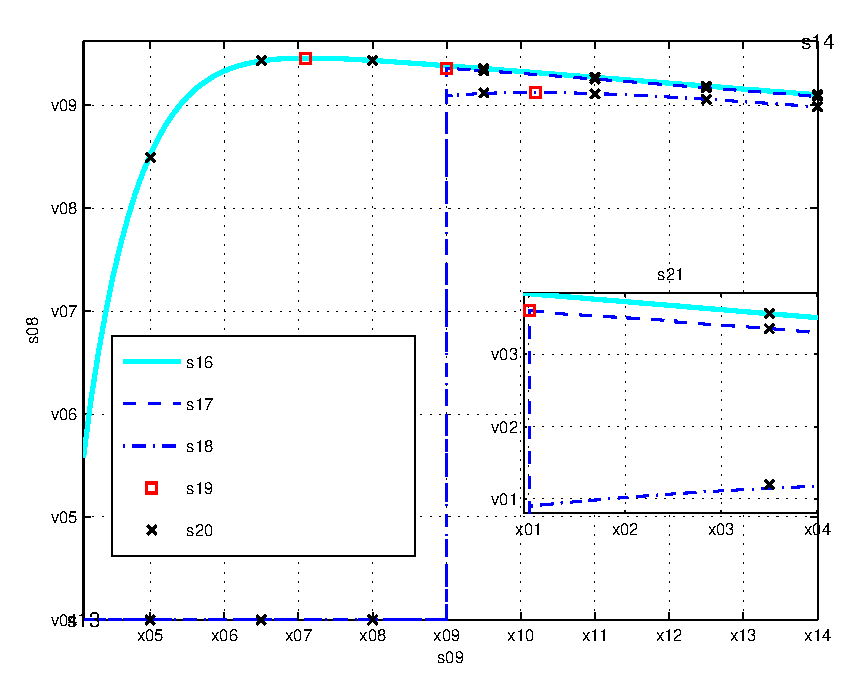
\includegraphics{fig_thr_sen_time_tradeoff_AWGN.eps}}%
%\end{psfrags}%
%
% End fig_thr_sen_time_tradeoff_AWGN.tex
\end{document}
% See http://www.mathworks.de/matlabcentral/fileexchange/loadFile.do?objectId=4638
% for recent versions of laprint.m.
%
% created by:           LaPrint version 3.16 (13.9.2004)
% created on:           12-Jul-2016 14:47:00
% eps bounding box:     16 cm x 12 cm
% comment:              
%
%\begin{psfrags}%
%\psfragscanon%
%
% text strings:
\psfrag{s08}[b][b]{\fontsize{8}{12}\fontseries{m}\mathversion{normal}\fontshape{n}\selectfont \color[rgb]{0,0,0}\setlength{\tabcolsep}{0pt}\begin{tabular}{c}$\rs(\test = \SI{5}{ms}, \tsen)$ [bits/sec/Hz]\end{tabular}}%
\psfrag{s09}[t][t]{\fontsize{8}{12}\fontseries{m}\mathversion{normal}\fontshape{n}\selectfont \color[rgb]{0,0,0}\setlength{\tabcolsep}{0pt}\begin{tabular}{c}$\tsen$ [ms]\end{tabular}}%
\psfrag{s13}[][]{\fontsize{10}{15}\fontseries{m}\mathversion{normal}\fontshape{n}\selectfont \color[rgb]{0,0,0}\setlength{\tabcolsep}{0pt}\begin{tabular}{c} \end{tabular}}%
\psfrag{s14}[][]{\fontsize{10}{15}\fontseries{m}\mathversion{normal}\fontshape{n}\selectfont \color[rgb]{0,0,0}\setlength{\tabcolsep}{0pt}\begin{tabular}{c} \end{tabular}}%
\psfrag{s15}[l][l]{\fontsize{8}{12}\fontseries{m}\mathversion{normal}\fontshape{n}\selectfont \color[rgb]{0,0,0}Simulated}%
\psfrag{s16}[l][l]{\fontsize{8}{12}\fontseries{m}\mathversion{normal}\fontshape{n}\selectfont \color[rgb]{0,0,0}IM}%
\psfrag{s17}[l][l]{\fontsize{8}{12}\fontseries{m}\mathversion{normal}\fontshape{n}\selectfont \color[rgb]{0,0,0}EM-AC, Problem 1}%
\psfrag{s18}[l][l]{\fontsize{8}{12}\fontseries{m}\mathversion{normal}\fontshape{n}\selectfont \color[rgb]{0,0,0}EM-OC, Problem 2}%
\psfrag{s19}[l][l]{\fontsize{8}{12}\fontseries{m}\mathversion{normal}\fontshape{n}\selectfont \color[rgb]{0,0,0}$\trs(\test,\ttsen)$}%
\psfrag{s20}[l][l]{\fontsize{8}{12}\fontseries{m}\mathversion{normal}\fontshape{n}\selectfont \color[rgb]{0,0,0}Simulated}%
\psfrag{s21}[b][b]{\fontsize{8}{12}\fontseries{m}\mathversion{normal}\fontshape{n}\selectfont \color[rgb]{0,0,0}\setlength{\tabcolsep}{0pt}\begin{tabular}{c}Zoom\end{tabular}}%
%
% axes font properties:
\fontsize{8}{12}\fontseries{m}\mathversion{normal}%
\fontshape{n}\selectfont%
%
% xticklabels:
\psfrag{x01}[t][t]{5}%
\psfrag{x02}[t][t]{5.2}%
\psfrag{x03}[t][t]{5.4}%
\psfrag{x04}[t][t]{5.6}%
\psfrag{x05}[t][t]{1}%
\psfrag{x06}[t][t]{2}%
\psfrag{x07}[t][t]{3}%
\psfrag{x08}[t][t]{4}%
\psfrag{x09}[t][t]{5}%
\psfrag{x10}[t][t]{6}%
\psfrag{x11}[t][t]{7}%
\psfrag{x12}[t][t]{8}%
\psfrag{x13}[t][t]{9}%
\psfrag{x14}[t][t]{10}%
%
% yticklabels:
\psfrag{v01}[r][r]{2.55}%
\psfrag{v02}[r][r]{2.6}%
\psfrag{v03}[r][r]{2.65}%
\psfrag{v04}[r][r]{0}%
\psfrag{v05}[r][r]{0.5}%
\psfrag{v06}[r][r]{1}%
\psfrag{v07}[r][r]{1.5}%
\psfrag{v08}[r][r]{2}%
\psfrag{v09}[r][r]{2.5}%
%
% Figure:
%\resizebox{8cm}{!}{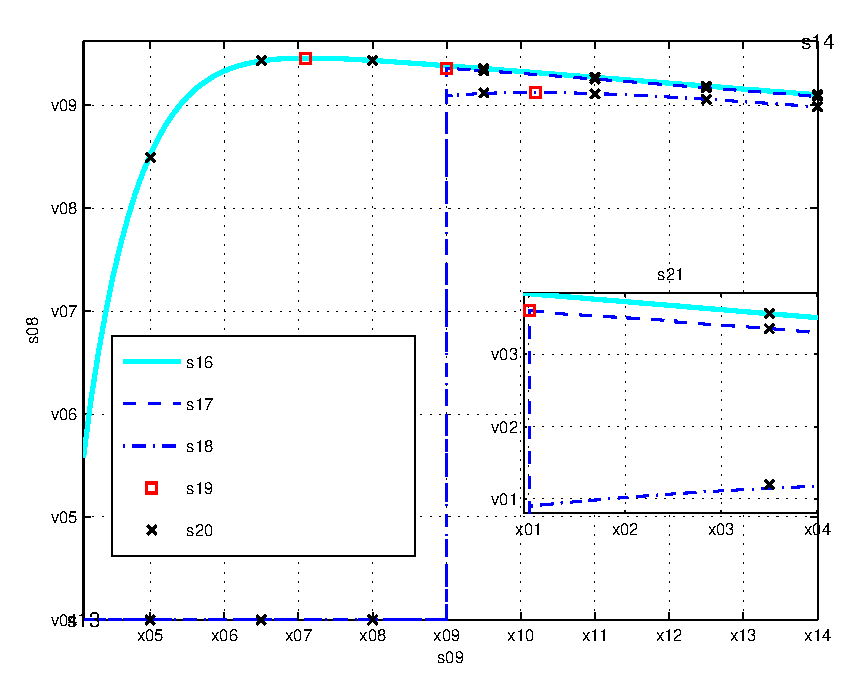
\includegraphics{fig_thr_sen_time_tradeoff_AWGN.eps}}%
%\end{psfrags}%
%
% End fig_thr_sen_time_tradeoff_AWGN.tex
\end{document}
% See http://www.mathworks.de/matlabcentral/fileexchange/loadFile.do?objectId=4638
% for recent versions of laprint.m.
%
% created by:           LaPrint version 3.16 (13.9.2004)
% created on:           12-Jul-2016 14:47:00
% eps bounding box:     16 cm x 12 cm
% comment:              
%
%\begin{psfrags}%
%\psfragscanon%
%
% text strings:
\psfrag{s08}[b][b]{\fontsize{8}{12}\fontseries{m}\mathversion{normal}\fontshape{n}\selectfont \color[rgb]{0,0,0}\setlength{\tabcolsep}{0pt}\begin{tabular}{c}$\rs(\test = \SI{5}{ms}, \tsen)$ [bits/sec/Hz]\end{tabular}}%
\psfrag{s09}[t][t]{\fontsize{8}{12}\fontseries{m}\mathversion{normal}\fontshape{n}\selectfont \color[rgb]{0,0,0}\setlength{\tabcolsep}{0pt}\begin{tabular}{c}$\tsen$ [ms]\end{tabular}}%
\psfrag{s13}[][]{\fontsize{10}{15}\fontseries{m}\mathversion{normal}\fontshape{n}\selectfont \color[rgb]{0,0,0}\setlength{\tabcolsep}{0pt}\begin{tabular}{c} \end{tabular}}%
\psfrag{s14}[][]{\fontsize{10}{15}\fontseries{m}\mathversion{normal}\fontshape{n}\selectfont \color[rgb]{0,0,0}\setlength{\tabcolsep}{0pt}\begin{tabular}{c} \end{tabular}}%
\psfrag{s15}[l][l]{\fontsize{8}{12}\fontseries{m}\mathversion{normal}\fontshape{n}\selectfont \color[rgb]{0,0,0}Simulated}%
\psfrag{s16}[l][l]{\fontsize{8}{12}\fontseries{m}\mathversion{normal}\fontshape{n}\selectfont \color[rgb]{0,0,0}IM}%
\psfrag{s17}[l][l]{\fontsize{8}{12}\fontseries{m}\mathversion{normal}\fontshape{n}\selectfont \color[rgb]{0,0,0}EM-AC, Problem 1}%
\psfrag{s18}[l][l]{\fontsize{8}{12}\fontseries{m}\mathversion{normal}\fontshape{n}\selectfont \color[rgb]{0,0,0}EM-OC, Problem 2}%
\psfrag{s19}[l][l]{\fontsize{8}{12}\fontseries{m}\mathversion{normal}\fontshape{n}\selectfont \color[rgb]{0,0,0}$\trs(\test,\ttsen)$}%
\psfrag{s20}[l][l]{\fontsize{8}{12}\fontseries{m}\mathversion{normal}\fontshape{n}\selectfont \color[rgb]{0,0,0}Simulated}%
\psfrag{s21}[b][b]{\fontsize{8}{12}\fontseries{m}\mathversion{normal}\fontshape{n}\selectfont \color[rgb]{0,0,0}\setlength{\tabcolsep}{0pt}\begin{tabular}{c}Zoom\end{tabular}}%
%
% axes font properties:
\fontsize{8}{12}\fontseries{m}\mathversion{normal}%
\fontshape{n}\selectfont%
%
% xticklabels:
\psfrag{x01}[t][t]{5}%
\psfrag{x02}[t][t]{5.2}%
\psfrag{x03}[t][t]{5.4}%
\psfrag{x04}[t][t]{5.6}%
\psfrag{x05}[t][t]{1}%
\psfrag{x06}[t][t]{2}%
\psfrag{x07}[t][t]{3}%
\psfrag{x08}[t][t]{4}%
\psfrag{x09}[t][t]{5}%
\psfrag{x10}[t][t]{6}%
\psfrag{x11}[t][t]{7}%
\psfrag{x12}[t][t]{8}%
\psfrag{x13}[t][t]{9}%
\psfrag{x14}[t][t]{10}%
%
% yticklabels:
\psfrag{v01}[r][r]{2.55}%
\psfrag{v02}[r][r]{2.6}%
\psfrag{v03}[r][r]{2.65}%
\psfrag{v04}[r][r]{0}%
\psfrag{v05}[r][r]{0.5}%
\psfrag{v06}[r][r]{1}%
\psfrag{v07}[r][r]{1.5}%
\psfrag{v08}[r][r]{2}%
\psfrag{v09}[r][r]{2.5}%
%
% Figure:
%\resizebox{8cm}{!}{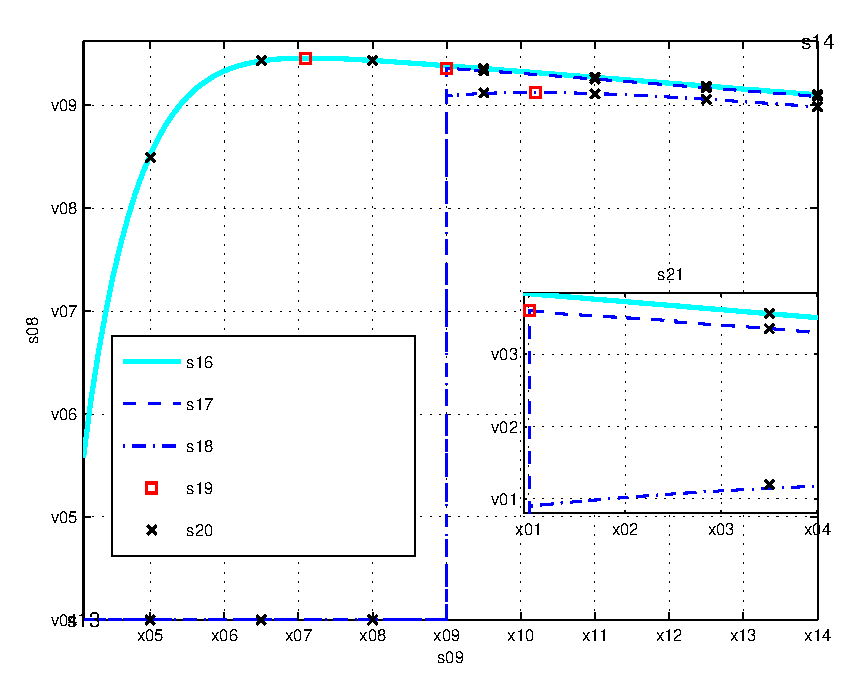
\includegraphics{fig_thr_sen_time_tradeoff_AWGN.eps}}%
%\end{psfrags}%
%
% End fig_thr_sen_time_tradeoff_AWGN.tex

\centering
\begin{tikzpicture}[scale=1]
\node[anchor=south west,inner sep=0] (image) at (0,0)
{
	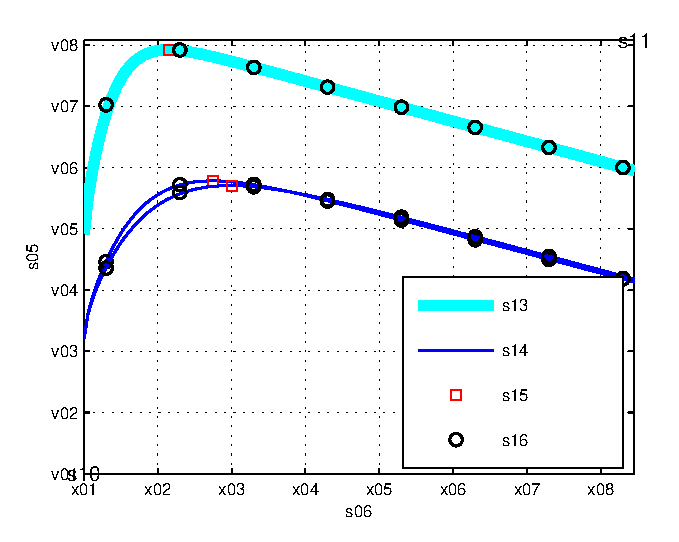
\includegraphics[width= \figscale]{figures/fig_thr_sen_time_tradeoff_AWGN}
};
\begin{scope}[x={(image.south east)},y={(image.north west)}]
\draw[black,thick,<->] (0.105,0.13) --  node[above, font=\small] {$\testpt = \testptsr = \testpr$} (0.16,0.13);

\draw[black,->] (0.23,0.53) -- (0.18,0.65);
\node[draw=none,font=\footnotesize] at (0.32,0.48) {$\opdc \in \{0.05,0.10\}$};

%\draw[help lines,xstep=.1,ystep=.1] (0,0) grid (1,1);
%\foreach \x in {0,1,...,9} { \node [anchor=north] at (\x/10,0) {0.\x}; }
%\foreach \y in {0,1,...,9} { \node [anchor=east] at (0,\y/10) {0.\y}; }
\end{scope}
\end{tikzpicture}
\caption{Sensing-throughput tradeoff for the Ideal Model and Estimation Model (EM) for $\testpt = \testptsr = \testpr = \SI{1}{ms}$.}
\label{fig:STT}
%\vspace{-0.7cm}
\end{figure}



\begin{figure}[!ht]
\vspace{-0.5cm}
%% Add psfrag entries
% This file is generated by the MATLAB m-file laprint.m. It can be included
% into LaTeX documents using the packages graphicx, color and psfrag.
% It is accompanied by a postscript file. A sample LaTeX file is:
%    \documentclass{article}\usepackage{graphicx,color,psfrag}
%    \begin{document}% This file is generated by the MATLAB m-file laprint.m. It can be included
% into LaTeX documents using the packages graphicx, color and psfrag.
% It is accompanied by a postscript file. A sample LaTeX file is:
%    \documentclass{article}\usepackage{graphicx,color,psfrag}
%    \begin{document}% This file is generated by the MATLAB m-file laprint.m. It can be included
% into LaTeX documents using the packages graphicx, color and psfrag.
% It is accompanied by a postscript file. A sample LaTeX file is:
%    \documentclass{article}\usepackage{graphicx,color,psfrag}
%    \begin{document}\input{fig_opt_thr_vs_SNR_AWGN}\end{document}
% See http://www.mathworks.de/matlabcentral/fileexchange/loadFile.do?objectId=4638
% for recent versions of laprint.m.
%
% created by:           LaPrint version 3.16 (13.9.2004)
% created on:           11-Oct-2015 14:32:29
% eps bounding box:     12 cm x 9 cm
% comment:              
%
%\begin{psfrags}%
%\psfragscanon%
%
% text strings:
\psfrag{s05}[b][b]{\fontsize{8}{12}\fontseries{m}\mathversion{normal}\fontshape{n}\selectfont \color[rgb]{0,0,0}\setlength{\tabcolsep}{0pt}\begin{tabular}{c}$\rs(\testpr,  \testpr, \ttsen)$ [bits/sec/Hz]\end{tabular}}%
\psfrag{s06}[t][t]{\fontsize{8}{12}\fontseries{m}\mathversion{normal}\fontshape{n}\selectfont \color[rgb]{0,0,0}\setlength{\tabcolsep}{0pt}\begin{tabular}{c}$\phpth$ [dB]\end{tabular}}%
\psfrag{s10}[][]{\fontsize{10}{15}\fontseries{m}\mathversion{normal}\fontshape{n}\selectfont \color[rgb]{0,0,0}\setlength{\tabcolsep}{0pt}\begin{tabular}{c} \end{tabular}}%
\psfrag{s11}[][]{\fontsize{10}{15}\fontseries{m}\mathversion{normal}\fontshape{n}\selectfont \color[rgb]{0,0,0}\setlength{\tabcolsep}{0pt}\begin{tabular}{c} \end{tabular}}%
\psfrag{s12}[l][l]{\fontsize{8}{12}\fontseries{m}\mathversion{normal}\fontshape{n}\selectfont \color[rgb]{0,0,0}EM}%
\psfrag{s13}[l][l]{\fontsize{8}{12}\fontseries{m}\mathversion{normal}\fontshape{n}\selectfont \color[rgb]{0,0,0}IM}%
\psfrag{s14}[l][l]{\fontsize{8}{12}\fontseries{m}\mathversion{normal}\fontshape{n}\selectfont \color[rgb]{0,0,0}EM}%
%
% axes font properties:
\fontsize{8}{12}\fontseries{m}\mathversion{normal}%
\fontshape{n}\selectfont%
%
% xticklabels:
\psfrag{x01}[t][t]{-110}%
\psfrag{x02}[t][t]{-105}%
\psfrag{x03}[t][t]{-100}%
\psfrag{x04}[t][t]{-95}%
\psfrag{x05}[t][t]{-90}%
%
% yticklabels:
\psfrag{v01}[r][r]{2.2}%
\psfrag{v02}[r][r]{2.4}%
\psfrag{v03}[r][r]{2.6}%
\psfrag{v04}[r][r]{2.8}%
\psfrag{v05}[r][r]{3}%
\psfrag{v06}[r][r]{3.2}%
\psfrag{v07}[r][r]{3.4}%
%
% Figure:
%\resizebox{6cm}{!}{\includegraphics{fig_opt_thr_vs_SNR_AWGN.eps}}%
%\end{psfrags}%
%
% End fig_opt_thr_vs_SNR_AWGN.tex
\end{document}
% See http://www.mathworks.de/matlabcentral/fileexchange/loadFile.do?objectId=4638
% for recent versions of laprint.m.
%
% created by:           LaPrint version 3.16 (13.9.2004)
% created on:           11-Oct-2015 14:32:29
% eps bounding box:     12 cm x 9 cm
% comment:              
%
%\begin{psfrags}%
%\psfragscanon%
%
% text strings:
\psfrag{s05}[b][b]{\fontsize{8}{12}\fontseries{m}\mathversion{normal}\fontshape{n}\selectfont \color[rgb]{0,0,0}\setlength{\tabcolsep}{0pt}\begin{tabular}{c}$\rs(\testpr,  \testpr, \ttsen)$ [bits/sec/Hz]\end{tabular}}%
\psfrag{s06}[t][t]{\fontsize{8}{12}\fontseries{m}\mathversion{normal}\fontshape{n}\selectfont \color[rgb]{0,0,0}\setlength{\tabcolsep}{0pt}\begin{tabular}{c}$\phpth$ [dB]\end{tabular}}%
\psfrag{s10}[][]{\fontsize{10}{15}\fontseries{m}\mathversion{normal}\fontshape{n}\selectfont \color[rgb]{0,0,0}\setlength{\tabcolsep}{0pt}\begin{tabular}{c} \end{tabular}}%
\psfrag{s11}[][]{\fontsize{10}{15}\fontseries{m}\mathversion{normal}\fontshape{n}\selectfont \color[rgb]{0,0,0}\setlength{\tabcolsep}{0pt}\begin{tabular}{c} \end{tabular}}%
\psfrag{s12}[l][l]{\fontsize{8}{12}\fontseries{m}\mathversion{normal}\fontshape{n}\selectfont \color[rgb]{0,0,0}EM}%
\psfrag{s13}[l][l]{\fontsize{8}{12}\fontseries{m}\mathversion{normal}\fontshape{n}\selectfont \color[rgb]{0,0,0}IM}%
\psfrag{s14}[l][l]{\fontsize{8}{12}\fontseries{m}\mathversion{normal}\fontshape{n}\selectfont \color[rgb]{0,0,0}EM}%
%
% axes font properties:
\fontsize{8}{12}\fontseries{m}\mathversion{normal}%
\fontshape{n}\selectfont%
%
% xticklabels:
\psfrag{x01}[t][t]{-110}%
\psfrag{x02}[t][t]{-105}%
\psfrag{x03}[t][t]{-100}%
\psfrag{x04}[t][t]{-95}%
\psfrag{x05}[t][t]{-90}%
%
% yticklabels:
\psfrag{v01}[r][r]{2.2}%
\psfrag{v02}[r][r]{2.4}%
\psfrag{v03}[r][r]{2.6}%
\psfrag{v04}[r][r]{2.8}%
\psfrag{v05}[r][r]{3}%
\psfrag{v06}[r][r]{3.2}%
\psfrag{v07}[r][r]{3.4}%
%
% Figure:
%\resizebox{6cm}{!}{\includegraphics{fig_opt_thr_vs_SNR_AWGN.eps}}%
%\end{psfrags}%
%
% End fig_opt_thr_vs_SNR_AWGN.tex
\end{document}
% See http://www.mathworks.de/matlabcentral/fileexchange/loadFile.do?objectId=4638
% for recent versions of laprint.m.
%
% created by:           LaPrint version 3.16 (13.9.2004)
% created on:           11-Oct-2015 14:32:29
% eps bounding box:     12 cm x 9 cm
% comment:              
%
%\begin{psfrags}%
%\psfragscanon%
%
% text strings:
\psfrag{s05}[b][b]{\fontsize{8}{12}\fontseries{m}\mathversion{normal}\fontshape{n}\selectfont \color[rgb]{0,0,0}\setlength{\tabcolsep}{0pt}\begin{tabular}{c}$\rs(\testpr,  \testpr, \ttsen)$ [bits/sec/Hz]\end{tabular}}%
\psfrag{s06}[t][t]{\fontsize{8}{12}\fontseries{m}\mathversion{normal}\fontshape{n}\selectfont \color[rgb]{0,0,0}\setlength{\tabcolsep}{0pt}\begin{tabular}{c}$\phpth$ [dB]\end{tabular}}%
\psfrag{s10}[][]{\fontsize{10}{15}\fontseries{m}\mathversion{normal}\fontshape{n}\selectfont \color[rgb]{0,0,0}\setlength{\tabcolsep}{0pt}\begin{tabular}{c} \end{tabular}}%
\psfrag{s11}[][]{\fontsize{10}{15}\fontseries{m}\mathversion{normal}\fontshape{n}\selectfont \color[rgb]{0,0,0}\setlength{\tabcolsep}{0pt}\begin{tabular}{c} \end{tabular}}%
\psfrag{s12}[l][l]{\fontsize{8}{12}\fontseries{m}\mathversion{normal}\fontshape{n}\selectfont \color[rgb]{0,0,0}EM}%
\psfrag{s13}[l][l]{\fontsize{8}{12}\fontseries{m}\mathversion{normal}\fontshape{n}\selectfont \color[rgb]{0,0,0}IM}%
\psfrag{s14}[l][l]{\fontsize{8}{12}\fontseries{m}\mathversion{normal}\fontshape{n}\selectfont \color[rgb]{0,0,0}EM}%
%
% axes font properties:
\fontsize{8}{12}\fontseries{m}\mathversion{normal}%
\fontshape{n}\selectfont%
%
% xticklabels:
\psfrag{x01}[t][t]{-110}%
\psfrag{x02}[t][t]{-105}%
\psfrag{x03}[t][t]{-100}%
\psfrag{x04}[t][t]{-95}%
\psfrag{x05}[t][t]{-90}%
%
% yticklabels:
\psfrag{v01}[r][r]{2.2}%
\psfrag{v02}[r][r]{2.4}%
\psfrag{v03}[r][r]{2.6}%
\psfrag{v04}[r][r]{2.8}%
\psfrag{v05}[r][r]{3}%
\psfrag{v06}[r][r]{3.2}%
\psfrag{v07}[r][r]{3.4}%
%
% Figure:
%\resizebox{6cm}{!}{\includegraphics{fig_opt_thr_vs_SNR_AWGN.eps}}%
%\end{psfrags}%
%
% End fig_opt_thr_vs_SNR_AWGN.tex

\centering
\begin{tikzpicture}[scale=1]
\node[anchor=south west,inner sep=0] (image) at (0,0)
{
	\includegraphics[width= \figscale]{figures/fig_opt_thr_vs_SNR_AWGN}
};
\begin{scope}[x={(image.south east)},y={(image.north west)}]
\draw[black,thick,<->] (0.82,0.18) --  node[below, font=\footnotesize] {Regime I} (0.955,0.18);
\draw[black,thick,<->] (0.39,0.18) --  node[below, font=\footnotesize] {Regime II} (0.815,0.18);
\draw[black,thick,<->] (0.11,0.18) --  node[below, font=\footnotesize] {Regime III} (0.385,0.18);
\draw[black,thick,<->] (0.28,0.235) --  node[above, rotate = 90, font=\footnotesize] {Performance Gain} (0.28,0.905);
\draw[black,thick,dashed,-] (0.27,0.232) -- (0.817,0.232);

%\draw[help lines,xstep=.1,ystep=.1] (0,0) grid (1,1);
%\foreach \x in {0,1,...,9} { \node [anchor=north] at (\x/10,0) {0.\x}; }
%\foreach \y in {0,1,...,9} { \node [anchor=east] at (0,\y/10) {0.\y}; }
\end{scope}
\end{tikzpicture}
\vspace{-0.2cm}
\caption{Achievable secondary throughput versus path loss $\phpth$ where the system is operating $\ttsen$ and the estimation time is fixed to $\testpt = \testptsr = \testpr = \SI{1}{ms}$.}
\label{fig:optT_SNR}
%\vspace{-0.8cm}
\end{figure}

\begin{figure}[!ht]
\vspace{-0.2cm}
%% Add psfrag entries
% This file is generated by the MATLAB m-file laprint.m. It can be included
% into LaTeX documents using the packages graphicx, color and psfrag.
% It is accompanied by a postscript file. A sample LaTeX file is:
%    \documentclass{article}\usepackage{graphicx,color,psfrag}
%    \begin{document}% This file is generated by the MATLAB m-file laprint.m. It can be included
% into LaTeX documents using the packages graphicx, color and psfrag.
% It is accompanied by a postscript file. A sample LaTeX file is:
%    \documentclass{article}\usepackage{graphicx,color,psfrag}
%    \begin{document}% This file is generated by the MATLAB m-file laprint.m. It can be included
% into LaTeX documents using the packages graphicx, color and psfrag.
% It is accompanied by a postscript file. A sample LaTeX file is:
%    \documentclass{article}\usepackage{graphicx,color,psfrag}
%    \begin{document}\input{fig_opt_cont_power_vs_SNR_AWGN}\end{document}
% See http://www.mathworks.de/matlabcentral/fileexchange/loadFile.do?objectId=4638
% for recent versions of laprint.m.
%
% created by:           LaPrint version 3.16 (13.9.2004)
% created on:           21-Feb-2016 20:15:44
% eps bounding box:     12 cm x 9 cm
% comment:              
%
%\begin{psfrags}%
%\psfragscanon%
%
% text strings:
\psfrag{s05}[b][b]{\fontsize{8}{12}\fontseries{m}\mathversion{normal}\fontshape{n}\selectfont \color[rgb]{0,0,0}\setlength{\tabcolsep}{0pt}\begin{tabular}{c}$\preg$ [dBm]\end{tabular}}%
\psfrag{s06}[t][t]{\fontsize{8}{12}\fontseries{m}\mathversion{normal}\fontshape{n}\selectfont \color[rgb]{0,0,0}\setlength{\tabcolsep}{0pt}\begin{tabular}{c}$\phpth$ [dB]\end{tabular}}%
\psfrag{s10}[][]{\fontsize{10}{15}\fontseries{m}\mathversion{normal}\fontshape{n}\selectfont \color[rgb]{0,0,0}\setlength{\tabcolsep}{0pt}\begin{tabular}{c} \end{tabular}}%
\psfrag{s11}[][]{\fontsize{10}{15}\fontseries{m}\mathversion{normal}\fontshape{n}\selectfont \color[rgb]{0,0,0}\setlength{\tabcolsep}{0pt}\begin{tabular}{c} \end{tabular}}%
\psfrag{s12}[l][l]{\fontsize{8}{12}\fontseries{m}\mathversion{normal}\fontshape{n}\selectfont \color[rgb]{0,0,0}EM}%
\psfrag{s13}[l][l]{\fontsize{8}{12}\fontseries{m}\mathversion{normal}\fontshape{n}\selectfont \color[rgb]{0,0,0}IM}%
\psfrag{s14}[l][l]{\fontsize{8}{12}\fontseries{m}\mathversion{normal}\fontshape{n}\selectfont \color[rgb]{0,0,0}EM}%
%
% axes font properties:
\fontsize{8}{12}\fontseries{m}\mathversion{normal}%
\fontshape{n}\selectfont%
%
% xticklabels:
\psfrag{x01}[t][t]{-110}%
\psfrag{x02}[t][t]{-105}%
\psfrag{x03}[t][t]{-100}%
\psfrag{x04}[t][t]{-95}%
\psfrag{x05}[t][t]{-90}%
%
% yticklabels:
\psfrag{v01}[r][r]{-20}%
\psfrag{v02}[r][r]{-15}%
\psfrag{v03}[r][r]{-10}%
\psfrag{v04}[r][r]{-5}%
\psfrag{v05}[r][r]{0}%
%
% Figure:
%\resizebox{6cm}{!}{\includegraphics{fig_opt_cont_power_vs_SNR_AWGN.eps}}%
%\end{psfrags}%
%
% End fig_opt_cont_power_vs_SNR_AWGN.tex
\end{document}
% See http://www.mathworks.de/matlabcentral/fileexchange/loadFile.do?objectId=4638
% for recent versions of laprint.m.
%
% created by:           LaPrint version 3.16 (13.9.2004)
% created on:           21-Feb-2016 20:15:44
% eps bounding box:     12 cm x 9 cm
% comment:              
%
%\begin{psfrags}%
%\psfragscanon%
%
% text strings:
\psfrag{s05}[b][b]{\fontsize{8}{12}\fontseries{m}\mathversion{normal}\fontshape{n}\selectfont \color[rgb]{0,0,0}\setlength{\tabcolsep}{0pt}\begin{tabular}{c}$\preg$ [dBm]\end{tabular}}%
\psfrag{s06}[t][t]{\fontsize{8}{12}\fontseries{m}\mathversion{normal}\fontshape{n}\selectfont \color[rgb]{0,0,0}\setlength{\tabcolsep}{0pt}\begin{tabular}{c}$\phpth$ [dB]\end{tabular}}%
\psfrag{s10}[][]{\fontsize{10}{15}\fontseries{m}\mathversion{normal}\fontshape{n}\selectfont \color[rgb]{0,0,0}\setlength{\tabcolsep}{0pt}\begin{tabular}{c} \end{tabular}}%
\psfrag{s11}[][]{\fontsize{10}{15}\fontseries{m}\mathversion{normal}\fontshape{n}\selectfont \color[rgb]{0,0,0}\setlength{\tabcolsep}{0pt}\begin{tabular}{c} \end{tabular}}%
\psfrag{s12}[l][l]{\fontsize{8}{12}\fontseries{m}\mathversion{normal}\fontshape{n}\selectfont \color[rgb]{0,0,0}EM}%
\psfrag{s13}[l][l]{\fontsize{8}{12}\fontseries{m}\mathversion{normal}\fontshape{n}\selectfont \color[rgb]{0,0,0}IM}%
\psfrag{s14}[l][l]{\fontsize{8}{12}\fontseries{m}\mathversion{normal}\fontshape{n}\selectfont \color[rgb]{0,0,0}EM}%
%
% axes font properties:
\fontsize{8}{12}\fontseries{m}\mathversion{normal}%
\fontshape{n}\selectfont%
%
% xticklabels:
\psfrag{x01}[t][t]{-110}%
\psfrag{x02}[t][t]{-105}%
\psfrag{x03}[t][t]{-100}%
\psfrag{x04}[t][t]{-95}%
\psfrag{x05}[t][t]{-90}%
%
% yticklabels:
\psfrag{v01}[r][r]{-20}%
\psfrag{v02}[r][r]{-15}%
\psfrag{v03}[r][r]{-10}%
\psfrag{v04}[r][r]{-5}%
\psfrag{v05}[r][r]{0}%
%
% Figure:
%\resizebox{6cm}{!}{\includegraphics{fig_opt_cont_power_vs_SNR_AWGN.eps}}%
%\end{psfrags}%
%
% End fig_opt_cont_power_vs_SNR_AWGN.tex
\end{document}
% See http://www.mathworks.de/matlabcentral/fileexchange/loadFile.do?objectId=4638
% for recent versions of laprint.m.
%
% created by:           LaPrint version 3.16 (13.9.2004)
% created on:           21-Feb-2016 20:15:44
% eps bounding box:     12 cm x 9 cm
% comment:              
%
%\begin{psfrags}%
%\psfragscanon%
%
% text strings:
\psfrag{s05}[b][b]{\fontsize{8}{12}\fontseries{m}\mathversion{normal}\fontshape{n}\selectfont \color[rgb]{0,0,0}\setlength{\tabcolsep}{0pt}\begin{tabular}{c}$\preg$ [dBm]\end{tabular}}%
\psfrag{s06}[t][t]{\fontsize{8}{12}\fontseries{m}\mathversion{normal}\fontshape{n}\selectfont \color[rgb]{0,0,0}\setlength{\tabcolsep}{0pt}\begin{tabular}{c}$\phpth$ [dB]\end{tabular}}%
\psfrag{s10}[][]{\fontsize{10}{15}\fontseries{m}\mathversion{normal}\fontshape{n}\selectfont \color[rgb]{0,0,0}\setlength{\tabcolsep}{0pt}\begin{tabular}{c} \end{tabular}}%
\psfrag{s11}[][]{\fontsize{10}{15}\fontseries{m}\mathversion{normal}\fontshape{n}\selectfont \color[rgb]{0,0,0}\setlength{\tabcolsep}{0pt}\begin{tabular}{c} \end{tabular}}%
\psfrag{s12}[l][l]{\fontsize{8}{12}\fontseries{m}\mathversion{normal}\fontshape{n}\selectfont \color[rgb]{0,0,0}EM}%
\psfrag{s13}[l][l]{\fontsize{8}{12}\fontseries{m}\mathversion{normal}\fontshape{n}\selectfont \color[rgb]{0,0,0}IM}%
\psfrag{s14}[l][l]{\fontsize{8}{12}\fontseries{m}\mathversion{normal}\fontshape{n}\selectfont \color[rgb]{0,0,0}EM}%
%
% axes font properties:
\fontsize{8}{12}\fontseries{m}\mathversion{normal}%
\fontshape{n}\selectfont%
%
% xticklabels:
\psfrag{x01}[t][t]{-110}%
\psfrag{x02}[t][t]{-105}%
\psfrag{x03}[t][t]{-100}%
\psfrag{x04}[t][t]{-95}%
\psfrag{x05}[t][t]{-90}%
%
% yticklabels:
\psfrag{v01}[r][r]{-20}%
\psfrag{v02}[r][r]{-15}%
\psfrag{v03}[r][r]{-10}%
\psfrag{v04}[r][r]{-5}%
\psfrag{v05}[r][r]{0}%
%
% Figure:
%\resizebox{6cm}{!}{\includegraphics{fig_opt_cont_power_vs_SNR_AWGN.eps}}%
%\end{psfrags}%
%
% End fig_opt_cont_power_vs_SNR_AWGN.tex

\centering
\begin{tikzpicture}[scale=1]
\node[anchor=south west,inner sep=0] (image) at (0,0)
{
\includegraphics[width= \figscale]{figures/fig_opt_cont_power_vs_SNR_AWGN}
};
\begin{scope}[x={(image.south east)},y={(image.north west)}]
\draw[black,thick,<->] (0.82,0.18) --  node[below, font=\footnotesize] {Regime I} (0.955,0.18);
\draw[black,thick,<->] (0.39,0.18) --  node[below, font=\footnotesize] {Regime II} (0.815,0.18);
\draw[black,thick,<->] (0.11,0.18) --  node[below, font=\footnotesize] {Regime III} (0.385,0.18);

%\draw[help lines,xstep=.1,ystep=.1] (0,0) grid (1,1);
%\foreach \x in {0,1,...,9} { \node [anchor=north] at (\x/10,0) {0.\x}; }
%\foreach \y in {0,1,...,9} { \node [anchor=east] at (0,\y/10) {0.\y}; }
\end{scope}
\end{tikzpicture}
\vspace{-0.2cm}
\caption{Optimim power control versus path loss $\phpth$ where the system is operating at $\ttsen$ and the estimation time is fixed to $\testpt = \testptsr = \testpr = \SI{1}{ms}$.}
\label{fig:optPcont_SNR}
%\vspace{-0.45cm}
\end{figure}

Following the previous discussions, it is well-known that the combination of interweave and underlay systems is intended to enhance the performance of the HS, hence, it is worthy to acquire insights on the performance gain in terms of the achievable secondary throughput due to the association of the underlay and the interweave techniques in the HS. In this regard, it is essential to observe the variations of the achievable secondary throughput corresponding to the interference channel from the ST to the PR, cf. \figurename~\ref{fig:scenario}. Before proceeding with the analysis, it is essential to understand that the performance of the underlay system decreases with the increase in the channel gain $\phpth$ \cite{Kaushik16_CL}. To simplify the analysis, the channel gain $\phpth \in [-110, -90] \SI{}{dBm}$ is categorized in three different regimes: (i) Regime I, (ii) Regime II and (iii) Regime III, cf. \figurename~\ref{fig:optT_SNR}. Under Regime I, large channel gain $\phpth > -\SI{93}{dB}$ causes control power to fall below a certain level $\preg \le \SI{-20}{dBm}$, cf. \figurename~\ref{fig:optPcont_SNR}, for the considered value of the channel gain $\phs = \SI{-80}{dB}$ over the access channel, such a low power transmission do not translate to an effective performance gain to the HS. As a result, no benefits are attained from the underlay system while operating in this regime, hence, the HS operates as an interweave system. In contrast to that, the Regime II ($-\SI{103}{dB} < \phpth < -\SI{93}{dB}$) witnesses a significant performance gain as HS procures benefits from both underlay and interweave systems. Moreover, it is observed that, no performance gain is attained below a certain channel gain $\phpth < \SI{-103}{dB}$ (Regime III). This is due to the fact that the ST is limited by the maximum transmit power, i.e., beyond $\SI{-103}{dB}$, $\preg = \pfull$, as illustrated in \figurename~\ref{fig:optPcont_SNR}. From this discussion, it can be concluded that the interference tolerance capability of the underlay system and the detection capability of the interweave system incorporated by the HS can be transformed into significant performance gain only in situations where channel to the PR is below a certain level, for instance $\phpth < -\SI{93}{dBm}$ for the considered case.



\begin{figure}[!t]
%% Add psfrag entries
% This file is generated by the MATLAB m-file laprint.m. It can be included
% into LaTeX documents using the packages graphicx, color and psfrag.
% It is accompanied by a postscript file. A sample LaTeX file is:
%    \documentclass{article}\usepackage{graphicx,color,psfrag}
%    \begin{document}% This file is generated by the MATLAB m-file laprint.m. It can be included
% into LaTeX documents using the packages graphicx, color and psfrag.
% It is accompanied by a postscript file. A sample LaTeX file is:
%    \documentclass{article}\usepackage{graphicx,color,psfrag}
%    \begin{document}% This file is generated by the MATLAB m-file laprint.m. It can be included
% into LaTeX documents using the packages graphicx, color and psfrag.
% It is accompanied by a postscript file. A sample LaTeX file is:
%    \documentclass{article}\usepackage{graphicx,color,psfrag}
%    \begin{document}\input{fig_opt_thr_vs_est_time_AWGN}\end{document}
% See http://www.mathworks.de/matlabcentral/fileexchange/loadFile.do?objectId=4638
% for recent versions of laprint.m.
%
% created by:           LaPrint version 3.16 (13.9.2004)
% created on:           04-Jul-2015 08:28:36
% eps bounding box:     16 cm x 12 cm
% comment:              
%
%\begin{psfrags}%
%\psfragscanon%
%
% text strings:
\psfrag{s05}[b][b]{\fontsize{9}{13.5}\fontseries{m}\mathversion{normal}\fontshape{n}\selectfont \color[rgb]{0,0,0}\setlength{\tabcolsep}{0pt}\begin{tabular}{c}$\trs$ [bits/sec/Hz]\end{tabular}}%
\psfrag{s06}[t][t]{\fontsize{9}{13.5}\fontseries{m}\mathversion{normal}\fontshape{n}\selectfont \color[rgb]{0,0,0}\setlength{\tabcolsep}{0pt}\begin{tabular}{c}$\test$ [ms]\end{tabular}}%
\psfrag{s10}[][]{\fontsize{10}{15}\fontseries{m}\mathversion{normal}\fontshape{n}\selectfont \color[rgb]{0,0,0}\setlength{\tabcolsep}{0pt}\begin{tabular}{c} \end{tabular}}%
\psfrag{s11}[][]{\fontsize{10}{15}\fontseries{m}\mathversion{normal}\fontshape{n}\selectfont \color[rgb]{0,0,0}\setlength{\tabcolsep}{0pt}\begin{tabular}{c} \end{tabular}}%
\psfrag{s12}[l][l]{\fontsize{9}{13.5}\fontseries{m}\mathversion{normal}\fontshape{n}\selectfont \color[rgb]{0,0,0}Opt. $\ttest$}%
\psfrag{s13}[l][l]{\fontsize{9}{13.5}\fontseries{m}\mathversion{normal}\fontshape{n}\selectfont \color[rgb]{0,0,0}$\trs$}%
\psfrag{s14}[l][l]{\fontsize{9}{13.5}\fontseries{m}\mathversion{normal}\fontshape{n}\selectfont \color[rgb]{0,0,0}$\trsac$}%
\psfrag{s15}[l][l]{\fontsize{9}{13.5}\fontseries{m}\mathversion{normal}\fontshape{n}\selectfont \color[rgb]{0,0,0}$\trsoc$}%
\psfrag{s16}[l][l]{\fontsize{9}{13.5}\fontseries{m}\mathversion{normal}\fontshape{n}\selectfont \color[rgb]{0,0,0}Opt. $\ttest$}%
%
% axes font properties:
\fontsize{9}{13.5}\fontseries{m}\mathversion{normal}%
\fontshape{n}\selectfont%
%
% xticklabels:
\psfrag{x01}[t][t]{1}%
\psfrag{x02}[t][t]{2}%
\psfrag{x03}[t][t]{3}%
\psfrag{x04}[t][t]{4}%
\psfrag{x05}[t][t]{5}%
\psfrag{x06}[t][t]{6}%
\psfrag{x07}[t][t]{7}%
\psfrag{x08}[t][t]{8}%
\psfrag{x09}[t][t]{9}%
\psfrag{x10}[t][t]{10}%
%
% yticklabels:
\psfrag{v01}[r][r]{0.5}%
\psfrag{v02}[r][r]{1}%
\psfrag{v03}[r][r]{1.5}%
\psfrag{v04}[r][r]{2}%
\psfrag{v05}[r][r]{2.5}%
%
% Figure:
%\resizebox{8cm}{!}{\includegraphics{fig_opt_thr_vs_est_time_AWGN.eps}}%
%\end{psfrags}%
%
% End fig_opt_thr_vs_est_time_AWGN.tex
\end{document}
% See http://www.mathworks.de/matlabcentral/fileexchange/loadFile.do?objectId=4638
% for recent versions of laprint.m.
%
% created by:           LaPrint version 3.16 (13.9.2004)
% created on:           04-Jul-2015 08:28:36
% eps bounding box:     16 cm x 12 cm
% comment:              
%
%\begin{psfrags}%
%\psfragscanon%
%
% text strings:
\psfrag{s05}[b][b]{\fontsize{9}{13.5}\fontseries{m}\mathversion{normal}\fontshape{n}\selectfont \color[rgb]{0,0,0}\setlength{\tabcolsep}{0pt}\begin{tabular}{c}$\trs$ [bits/sec/Hz]\end{tabular}}%
\psfrag{s06}[t][t]{\fontsize{9}{13.5}\fontseries{m}\mathversion{normal}\fontshape{n}\selectfont \color[rgb]{0,0,0}\setlength{\tabcolsep}{0pt}\begin{tabular}{c}$\test$ [ms]\end{tabular}}%
\psfrag{s10}[][]{\fontsize{10}{15}\fontseries{m}\mathversion{normal}\fontshape{n}\selectfont \color[rgb]{0,0,0}\setlength{\tabcolsep}{0pt}\begin{tabular}{c} \end{tabular}}%
\psfrag{s11}[][]{\fontsize{10}{15}\fontseries{m}\mathversion{normal}\fontshape{n}\selectfont \color[rgb]{0,0,0}\setlength{\tabcolsep}{0pt}\begin{tabular}{c} \end{tabular}}%
\psfrag{s12}[l][l]{\fontsize{9}{13.5}\fontseries{m}\mathversion{normal}\fontshape{n}\selectfont \color[rgb]{0,0,0}Opt. $\ttest$}%
\psfrag{s13}[l][l]{\fontsize{9}{13.5}\fontseries{m}\mathversion{normal}\fontshape{n}\selectfont \color[rgb]{0,0,0}$\trs$}%
\psfrag{s14}[l][l]{\fontsize{9}{13.5}\fontseries{m}\mathversion{normal}\fontshape{n}\selectfont \color[rgb]{0,0,0}$\trsac$}%
\psfrag{s15}[l][l]{\fontsize{9}{13.5}\fontseries{m}\mathversion{normal}\fontshape{n}\selectfont \color[rgb]{0,0,0}$\trsoc$}%
\psfrag{s16}[l][l]{\fontsize{9}{13.5}\fontseries{m}\mathversion{normal}\fontshape{n}\selectfont \color[rgb]{0,0,0}Opt. $\ttest$}%
%
% axes font properties:
\fontsize{9}{13.5}\fontseries{m}\mathversion{normal}%
\fontshape{n}\selectfont%
%
% xticklabels:
\psfrag{x01}[t][t]{1}%
\psfrag{x02}[t][t]{2}%
\psfrag{x03}[t][t]{3}%
\psfrag{x04}[t][t]{4}%
\psfrag{x05}[t][t]{5}%
\psfrag{x06}[t][t]{6}%
\psfrag{x07}[t][t]{7}%
\psfrag{x08}[t][t]{8}%
\psfrag{x09}[t][t]{9}%
\psfrag{x10}[t][t]{10}%
%
% yticklabels:
\psfrag{v01}[r][r]{0.5}%
\psfrag{v02}[r][r]{1}%
\psfrag{v03}[r][r]{1.5}%
\psfrag{v04}[r][r]{2}%
\psfrag{v05}[r][r]{2.5}%
%
% Figure:
%\resizebox{8cm}{!}{\includegraphics{fig_opt_thr_vs_est_time_AWGN.eps}}%
%\end{psfrags}%
%
% End fig_opt_thr_vs_est_time_AWGN.tex
\end{document}
% See http://www.mathworks.de/matlabcentral/fileexchange/loadFile.do?objectId=4638
% for recent versions of laprint.m.
%
% created by:           LaPrint version 3.16 (13.9.2004)
% created on:           04-Jul-2015 08:28:36
% eps bounding box:     16 cm x 12 cm
% comment:              
%
%\begin{psfrags}%
%\psfragscanon%
%
% text strings:
\psfrag{s05}[b][b]{\fontsize{9}{13.5}\fontseries{m}\mathversion{normal}\fontshape{n}\selectfont \color[rgb]{0,0,0}\setlength{\tabcolsep}{0pt}\begin{tabular}{c}$\trs$ [bits/sec/Hz]\end{tabular}}%
\psfrag{s06}[t][t]{\fontsize{9}{13.5}\fontseries{m}\mathversion{normal}\fontshape{n}\selectfont \color[rgb]{0,0,0}\setlength{\tabcolsep}{0pt}\begin{tabular}{c}$\test$ [ms]\end{tabular}}%
\psfrag{s10}[][]{\fontsize{10}{15}\fontseries{m}\mathversion{normal}\fontshape{n}\selectfont \color[rgb]{0,0,0}\setlength{\tabcolsep}{0pt}\begin{tabular}{c} \end{tabular}}%
\psfrag{s11}[][]{\fontsize{10}{15}\fontseries{m}\mathversion{normal}\fontshape{n}\selectfont \color[rgb]{0,0,0}\setlength{\tabcolsep}{0pt}\begin{tabular}{c} \end{tabular}}%
\psfrag{s12}[l][l]{\fontsize{9}{13.5}\fontseries{m}\mathversion{normal}\fontshape{n}\selectfont \color[rgb]{0,0,0}Opt. $\ttest$}%
\psfrag{s13}[l][l]{\fontsize{9}{13.5}\fontseries{m}\mathversion{normal}\fontshape{n}\selectfont \color[rgb]{0,0,0}$\trs$}%
\psfrag{s14}[l][l]{\fontsize{9}{13.5}\fontseries{m}\mathversion{normal}\fontshape{n}\selectfont \color[rgb]{0,0,0}$\trsac$}%
\psfrag{s15}[l][l]{\fontsize{9}{13.5}\fontseries{m}\mathversion{normal}\fontshape{n}\selectfont \color[rgb]{0,0,0}$\trsoc$}%
\psfrag{s16}[l][l]{\fontsize{9}{13.5}\fontseries{m}\mathversion{normal}\fontshape{n}\selectfont \color[rgb]{0,0,0}Opt. $\ttest$}%
%
% axes font properties:
\fontsize{9}{13.5}\fontseries{m}\mathversion{normal}%
\fontshape{n}\selectfont%
%
% xticklabels:
\psfrag{x01}[t][t]{1}%
\psfrag{x02}[t][t]{2}%
\psfrag{x03}[t][t]{3}%
\psfrag{x04}[t][t]{4}%
\psfrag{x05}[t][t]{5}%
\psfrag{x06}[t][t]{6}%
\psfrag{x07}[t][t]{7}%
\psfrag{x08}[t][t]{8}%
\psfrag{x09}[t][t]{9}%
\psfrag{x10}[t][t]{10}%
%
% yticklabels:
\psfrag{v01}[r][r]{0.5}%
\psfrag{v02}[r][r]{1}%
\psfrag{v03}[r][r]{1.5}%
\psfrag{v04}[r][r]{2}%
\psfrag{v05}[r][r]{2.5}%
%
% Figure:
%\resizebox{8cm}{!}{\includegraphics{fig_opt_thr_vs_est_time_AWGN.eps}}%
%\end{psfrags}%
%
% End fig_opt_thr_vs_est_time_AWGN.tex

\centering
\begin{tikzpicture}[scale=1]
\node[anchor=south west,inner sep=0] (image) at (0,0)
{
\includegraphics[width= \figscale]{figures/fig_opt_thr_vs_est_time_AWGN}
};
\begin{scope}[x={(image.south east)},y={(image.north west)}]
\draw[black,->] (0.23,0.58) -- (0.18,0.68);
\node[draw=none,  ] at (0.34, 0.55) {$\opdc \in \{0.05,0.10\}$};

%\draw[help lines,xstep=.1,ystep=.1] (0,0) grid (1,1);
%\foreach \x in {0,1,...,9} { \node [anchor=north] at (\x/10,0) {0.\x}; }
%\foreach \y in {0,1,...,9} { \node [anchor=east] at (0,\y/10) {0.\y}; }
\end{scope}
\end{tikzpicture}
\caption{Achievable secondary throughput versus the estimation time $\testpt = \testptsr = \testpr$ operating at the suitable sensing time $\ttsen$.}
\label{fig:optT_est_time}
%\vspace{-0.45cm}
\end{figure}

Besides maximizing the secondary throughput over the sensing time, it is interesting to observe the variation of the achievable throughput with the estimation time.
%It is evident that $\testptsr$ contributes only to the variations in the capacities $\co, \cth$, since the system model considers their expected values, cf. (\ref{eq:exp_thr}), these variations does not have a significant impact on the achievable throughput. In this regard, we consider the variations due to $\testpt$ and $\testpr$ only. 
As proposed in Theorem \ref{th:th1}, $\testpt = \testptsr = \testpr$ is considered for the analysis. Corresponding to the estimation model, \figurename~\ref{fig:optT_est_time} reveals the estimation-sensing-throughput tradeoff, cf. Remark \ref{co:coro1}. This effect can be explained as follows, the variations due to the estimation of $\phpo$ and $\phpth$ causes variations in $\pd$ and $\eprcvdpr$, these variations are captured using the outage constraints, hence, a small increase in $\testpt$ $(= \testptsr = \testpr)$ leads to a significant performance improvement in terms of secondary throughput, however increasing the estimation time beyond $\ttestpt$ $(= \ttestptsr= \ttestpr)$ slightly contributes to the performance improvement and largely consumes the time resources. Moreover, it is noticed that performance degradation of the secondary system evaluated in terms of $\rs(\testpt$ $= \testptsr = \testpr, \ttsen)$ becomes more sensitive to the estimation time $\ttestpt$ $(= \ttestptsr= \ttestpr)$ as $\opdc$ decreases. From this, it can be concluded that a suitable choice of estimation time becomes significant, specially to those HS that are pertained to the aggressive policies provided by the primary systems or regulatory bodies. 


\begin{figure}[!t]
%\vspace{-0.8cm}
%% Add psfrag entries
% This file is generated by the MATLAB m-file laprint.m. It can be included
% into LaTeX documents using the packages graphicx, color and psfrag.
% It is accompanied by a postscript file. A sample LaTeX file is:
%    \documentclass{article}\usepackage{graphicx,color,psfrag}
%    \begin{document}% This file is generated by the MATLAB m-file laprint.m. It can be included
% into LaTeX documents using the packages graphicx, color and psfrag.
% It is accompanied by a postscript file. A sample LaTeX file is:
%    \documentclass{article}\usepackage{graphicx,color,psfrag}
%    \begin{document}% This file is generated by the MATLAB m-file laprint.m. It can be included
% into LaTeX documents using the packages graphicx, color and psfrag.
% It is accompanied by a postscript file. A sample LaTeX file is:
%    \documentclass{article}\usepackage{graphicx,color,psfrag}
%    \begin{document}\input{fig_P_d_vs_est_time_AWGN}\end{document}
% See http://www.mathworks.de/matlabcentral/fileexchange/loadFile.do?objectId=4638
% for recent versions of laprint.m.
%
% created by:           LaPrint version 3.16 (13.9.2004)
% created on:           11-Oct-2015 14:34:55
% eps bounding box:     12 cm x 9 cm
% comment:              
%
%\begin{psfrags}%
%\psfragscanon%
%
% text strings:
\psfrag{s05}[b][b]{\fontsize{8}{12}\fontseries{m}\mathversion{normal}\fontshape{n}\selectfont \color[rgb]{0,0,0}\setlength{\tabcolsep}{0pt}\begin{tabular}{c}$\e{\pd}{\pd}$\end{tabular}}%
\psfrag{s06}[t][t]{\fontsize{8}{12}\fontseries{m}\mathversion{normal}\fontshape{n}\selectfont \color[rgb]{0,0,0}\setlength{\tabcolsep}{0pt}\begin{tabular}{c}$\testpt = \testpr$  [ms]\end{tabular}}%
\psfrag{s10}[][]{\fontsize{10}{15}\fontseries{m}\mathversion{normal}\fontshape{n}\selectfont \color[rgb]{0,0,0}\setlength{\tabcolsep}{0pt}\begin{tabular}{c} \end{tabular}}%
\psfrag{s11}[][]{\fontsize{10}{15}\fontseries{m}\mathversion{normal}\fontshape{n}\selectfont \color[rgb]{0,0,0}\setlength{\tabcolsep}{0pt}\begin{tabular}{c} \end{tabular}}%
\psfrag{s12}[l][l]{\fontsize{8}{12}\fontseries{m}\mathversion{normal}\fontshape{n}\selectfont \color[rgb]{0,0,0}EM}%
\psfrag{s13}[l][l]{\fontsize{8}{12}\fontseries{m}\mathversion{normal}\fontshape{n}\selectfont \color[rgb]{0,0,0}IM}%
\psfrag{s14}[l][l]{\fontsize{8}{12}\fontseries{m}\mathversion{normal}\fontshape{n}\selectfont \color[rgb]{0,0,0}EM}%
%
% axes font properties:
\fontsize{8}{12}\fontseries{m}\mathversion{normal}%
\fontshape{n}\selectfont%
%
% xticklabels:
\psfrag{x01}[t][t]{1}%
\psfrag{x02}[t][t]{2}%
\psfrag{x03}[t][t]{3}%
\psfrag{x04}[t][t]{4}%
\psfrag{x05}[t][t]{5}%
\psfrag{x06}[t][t]{6}%
\psfrag{x07}[t][t]{7}%
\psfrag{x08}[t][t]{8}%
\psfrag{x09}[t][t]{9}%
\psfrag{x10}[t][t]{10}%
%
% yticklabels:
\psfrag{v01}[r][r]{0.8}%
\psfrag{v02}[r][r]{0.85}%
\psfrag{v03}[r][r]{0.9}%
\psfrag{v04}[r][r]{0.95}%
%
% Figure:
%\resizebox{6cm}{!}{\includegraphics{fig_P_d_vs_est_time_AWGN.eps}}%
%\end{psfrags}%
%
% End fig_P_d_vs_est_time_AWGN.tex
\end{document}
% See http://www.mathworks.de/matlabcentral/fileexchange/loadFile.do?objectId=4638
% for recent versions of laprint.m.
%
% created by:           LaPrint version 3.16 (13.9.2004)
% created on:           11-Oct-2015 14:34:55
% eps bounding box:     12 cm x 9 cm
% comment:              
%
%\begin{psfrags}%
%\psfragscanon%
%
% text strings:
\psfrag{s05}[b][b]{\fontsize{8}{12}\fontseries{m}\mathversion{normal}\fontshape{n}\selectfont \color[rgb]{0,0,0}\setlength{\tabcolsep}{0pt}\begin{tabular}{c}$\e{\pd}{\pd}$\end{tabular}}%
\psfrag{s06}[t][t]{\fontsize{8}{12}\fontseries{m}\mathversion{normal}\fontshape{n}\selectfont \color[rgb]{0,0,0}\setlength{\tabcolsep}{0pt}\begin{tabular}{c}$\testpt = \testpr$  [ms]\end{tabular}}%
\psfrag{s10}[][]{\fontsize{10}{15}\fontseries{m}\mathversion{normal}\fontshape{n}\selectfont \color[rgb]{0,0,0}\setlength{\tabcolsep}{0pt}\begin{tabular}{c} \end{tabular}}%
\psfrag{s11}[][]{\fontsize{10}{15}\fontseries{m}\mathversion{normal}\fontshape{n}\selectfont \color[rgb]{0,0,0}\setlength{\tabcolsep}{0pt}\begin{tabular}{c} \end{tabular}}%
\psfrag{s12}[l][l]{\fontsize{8}{12}\fontseries{m}\mathversion{normal}\fontshape{n}\selectfont \color[rgb]{0,0,0}EM}%
\psfrag{s13}[l][l]{\fontsize{8}{12}\fontseries{m}\mathversion{normal}\fontshape{n}\selectfont \color[rgb]{0,0,0}IM}%
\psfrag{s14}[l][l]{\fontsize{8}{12}\fontseries{m}\mathversion{normal}\fontshape{n}\selectfont \color[rgb]{0,0,0}EM}%
%
% axes font properties:
\fontsize{8}{12}\fontseries{m}\mathversion{normal}%
\fontshape{n}\selectfont%
%
% xticklabels:
\psfrag{x01}[t][t]{1}%
\psfrag{x02}[t][t]{2}%
\psfrag{x03}[t][t]{3}%
\psfrag{x04}[t][t]{4}%
\psfrag{x05}[t][t]{5}%
\psfrag{x06}[t][t]{6}%
\psfrag{x07}[t][t]{7}%
\psfrag{x08}[t][t]{8}%
\psfrag{x09}[t][t]{9}%
\psfrag{x10}[t][t]{10}%
%
% yticklabels:
\psfrag{v01}[r][r]{0.8}%
\psfrag{v02}[r][r]{0.85}%
\psfrag{v03}[r][r]{0.9}%
\psfrag{v04}[r][r]{0.95}%
%
% Figure:
%\resizebox{6cm}{!}{\includegraphics{fig_P_d_vs_est_time_AWGN.eps}}%
%\end{psfrags}%
%
% End fig_P_d_vs_est_time_AWGN.tex
\end{document}
% See http://www.mathworks.de/matlabcentral/fileexchange/loadFile.do?objectId=4638
% for recent versions of laprint.m.
%
% created by:           LaPrint version 3.16 (13.9.2004)
% created on:           11-Oct-2015 14:34:55
% eps bounding box:     12 cm x 9 cm
% comment:              
%
%\begin{psfrags}%
%\psfragscanon%
%
% text strings:
\psfrag{s05}[b][b]{\fontsize{8}{12}\fontseries{m}\mathversion{normal}\fontshape{n}\selectfont \color[rgb]{0,0,0}\setlength{\tabcolsep}{0pt}\begin{tabular}{c}$\e{\pd}{\pd}$\end{tabular}}%
\psfrag{s06}[t][t]{\fontsize{8}{12}\fontseries{m}\mathversion{normal}\fontshape{n}\selectfont \color[rgb]{0,0,0}\setlength{\tabcolsep}{0pt}\begin{tabular}{c}$\testpt = \testpr$  [ms]\end{tabular}}%
\psfrag{s10}[][]{\fontsize{10}{15}\fontseries{m}\mathversion{normal}\fontshape{n}\selectfont \color[rgb]{0,0,0}\setlength{\tabcolsep}{0pt}\begin{tabular}{c} \end{tabular}}%
\psfrag{s11}[][]{\fontsize{10}{15}\fontseries{m}\mathversion{normal}\fontshape{n}\selectfont \color[rgb]{0,0,0}\setlength{\tabcolsep}{0pt}\begin{tabular}{c} \end{tabular}}%
\psfrag{s12}[l][l]{\fontsize{8}{12}\fontseries{m}\mathversion{normal}\fontshape{n}\selectfont \color[rgb]{0,0,0}EM}%
\psfrag{s13}[l][l]{\fontsize{8}{12}\fontseries{m}\mathversion{normal}\fontshape{n}\selectfont \color[rgb]{0,0,0}IM}%
\psfrag{s14}[l][l]{\fontsize{8}{12}\fontseries{m}\mathversion{normal}\fontshape{n}\selectfont \color[rgb]{0,0,0}EM}%
%
% axes font properties:
\fontsize{8}{12}\fontseries{m}\mathversion{normal}%
\fontshape{n}\selectfont%
%
% xticklabels:
\psfrag{x01}[t][t]{1}%
\psfrag{x02}[t][t]{2}%
\psfrag{x03}[t][t]{3}%
\psfrag{x04}[t][t]{4}%
\psfrag{x05}[t][t]{5}%
\psfrag{x06}[t][t]{6}%
\psfrag{x07}[t][t]{7}%
\psfrag{x08}[t][t]{8}%
\psfrag{x09}[t][t]{9}%
\psfrag{x10}[t][t]{10}%
%
% yticklabels:
\psfrag{v01}[r][r]{0.8}%
\psfrag{v02}[r][r]{0.85}%
\psfrag{v03}[r][r]{0.9}%
\psfrag{v04}[r][r]{0.95}%
%
% Figure:
%\resizebox{6cm}{!}{\includegraphics{fig_P_d_vs_est_time_AWGN.eps}}%
%\end{psfrags}%
%
% End fig_P_d_vs_est_time_AWGN.tex

\centering
\begin{tikzpicture}[scale=1]
\node[anchor=south west,inner sep=0] (image) at (0,0)
{
\includegraphics[width= \figscale]{figures/fig_P_d_vs_est_time_AWGN}
};
\begin{scope}[x={(image.south east)},y={(image.north west)}]
\draw[black,<-] (0.28,0.72) -- (0.23,0.88);
\node[draw=none] at (0.3, 0.92) {$\opdc \in \{0.05,0.10\}$};

%\draw[help lines,xstep=.1,ystep=.1] (0,0) grid (1,1);
%\foreach \x in {0,1,...,9} { \node [anchor=north] at (\x/10,0) {0.\x}; }
%\foreach \y in {0,1,...,9} { \node [anchor=east] at (0,\y/10) {0.\y}; }
\end{scope}
\end{tikzpicture}
\caption{Detection probability versus $\testpt = \testptsr = \testpr$ operating at the suitable sensing time $\ttsen$.}
\label{fig:P_d_est_time}
%\vspace{-0.8cm}
\end{figure}

\begin{figure}[!t]
%% Add psfrag entries
% This file is generated by the MATLAB m-file laprint.m. It can be included
% into LaTeX documents using the packages graphicx, color and psfrag.
% It is accompanied by a postscript file. A sample LaTeX file is:
%    \documentclass{article}\usepackage{graphicx,color,psfrag}
%    \begin{document}% This file is generated by the MATLAB m-file laprint.m. It can be included
% into LaTeX documents using the packages graphicx, color and psfrag.
% It is accompanied by a postscript file. A sample LaTeX file is:
%    \documentclass{article}\usepackage{graphicx,color,psfrag}
%    \begin{document}% This file is generated by the MATLAB m-file laprint.m. It can be included
% into LaTeX documents using the packages graphicx, color and psfrag.
% It is accompanied by a postscript file. A sample LaTeX file is:
%    \documentclass{article}\usepackage{graphicx,color,psfrag}
%    \begin{document}\input{fig_P_f_vs_est_time_AWGN}\end{document}
% See http://www.mathworks.de/matlabcentral/fileexchange/loadFile.do?objectId=4638
% for recent versions of laprint.m.
%
% created by:           LaPrint version 3.16 (13.9.2004)
% created on:           11-Oct-2015 14:33:12
% eps bounding box:     12 cm x 9 cm
% comment:              
%
%\begin{psfrags}%
%\psfragscanon%
%
% text strings:
\psfrag{s05}[b][b]{\fontsize{8}{12}\fontseries{m}\mathversion{normal}\fontshape{n}\selectfont \color[rgb]{0,0,0}\setlength{\tabcolsep}{0pt}\begin{tabular}{c}$\pfa$\end{tabular}}%
\psfrag{s06}[t][t]{\fontsize{8}{12}\fontseries{m}\mathversion{normal}\fontshape{n}\selectfont \color[rgb]{0,0,0}\setlength{\tabcolsep}{0pt}\begin{tabular}{c}$\testpt = \testpr$  [ms]\end{tabular}}%
\psfrag{s10}[][]{\fontsize{10}{15}\fontseries{m}\mathversion{normal}\fontshape{n}\selectfont \color[rgb]{0,0,0}\setlength{\tabcolsep}{0pt}\begin{tabular}{c} \end{tabular}}%
\psfrag{s11}[][]{\fontsize{10}{15}\fontseries{m}\mathversion{normal}\fontshape{n}\selectfont \color[rgb]{0,0,0}\setlength{\tabcolsep}{0pt}\begin{tabular}{c} \end{tabular}}%
\psfrag{s12}[l][l]{\fontsize{8}{12}\fontseries{m}\mathversion{normal}\fontshape{n}\selectfont \color[rgb]{0,0,0}EM}%
\psfrag{s13}[l][l]{\fontsize{8}{12}\fontseries{m}\mathversion{normal}\fontshape{n}\selectfont \color[rgb]{0,0,0}IM}%
\psfrag{s14}[l][l]{\fontsize{8}{12}\fontseries{m}\mathversion{normal}\fontshape{n}\selectfont \color[rgb]{0,0,0}EM}%
%
% axes font properties:
\fontsize{8}{12}\fontseries{m}\mathversion{normal}%
\fontshape{n}\selectfont%
%
% xticklabels:
\psfrag{x01}[t][t]{1}%
\psfrag{x02}[t][t]{2}%
\psfrag{x03}[t][t]{3}%
\psfrag{x04}[t][t]{4}%
\psfrag{x05}[t][t]{5}%
\psfrag{x06}[t][t]{6}%
\psfrag{x07}[t][t]{7}%
\psfrag{x08}[t][t]{8}%
\psfrag{x09}[t][t]{9}%
\psfrag{x10}[t][t]{10}%
%
% yticklabels:
\psfrag{v01}[r][r]{0.05}%
\psfrag{v02}[r][r]{0.1}%
\psfrag{v03}[r][r]{0.15}%
\psfrag{v04}[r][r]{0.2}%
\psfrag{v05}[r][r]{0.25}%
\psfrag{v06}[r][r]{0.3}%
\psfrag{v07}[r][r]{0.35}%
\psfrag{v08}[r][r]{0.4}%
\psfrag{v09}[r][r]{0.45}%
%
% Figure:
%\resizebox{6cm}{!}{\includegraphics{fig_P_f_vs_est_time_AWGN.eps}}%
%\end{psfrags}%
%
% End fig_P_f_vs_est_time_AWGN.tex
\end{document}
% See http://www.mathworks.de/matlabcentral/fileexchange/loadFile.do?objectId=4638
% for recent versions of laprint.m.
%
% created by:           LaPrint version 3.16 (13.9.2004)
% created on:           11-Oct-2015 14:33:12
% eps bounding box:     12 cm x 9 cm
% comment:              
%
%\begin{psfrags}%
%\psfragscanon%
%
% text strings:
\psfrag{s05}[b][b]{\fontsize{8}{12}\fontseries{m}\mathversion{normal}\fontshape{n}\selectfont \color[rgb]{0,0,0}\setlength{\tabcolsep}{0pt}\begin{tabular}{c}$\pfa$\end{tabular}}%
\psfrag{s06}[t][t]{\fontsize{8}{12}\fontseries{m}\mathversion{normal}\fontshape{n}\selectfont \color[rgb]{0,0,0}\setlength{\tabcolsep}{0pt}\begin{tabular}{c}$\testpt = \testpr$  [ms]\end{tabular}}%
\psfrag{s10}[][]{\fontsize{10}{15}\fontseries{m}\mathversion{normal}\fontshape{n}\selectfont \color[rgb]{0,0,0}\setlength{\tabcolsep}{0pt}\begin{tabular}{c} \end{tabular}}%
\psfrag{s11}[][]{\fontsize{10}{15}\fontseries{m}\mathversion{normal}\fontshape{n}\selectfont \color[rgb]{0,0,0}\setlength{\tabcolsep}{0pt}\begin{tabular}{c} \end{tabular}}%
\psfrag{s12}[l][l]{\fontsize{8}{12}\fontseries{m}\mathversion{normal}\fontshape{n}\selectfont \color[rgb]{0,0,0}EM}%
\psfrag{s13}[l][l]{\fontsize{8}{12}\fontseries{m}\mathversion{normal}\fontshape{n}\selectfont \color[rgb]{0,0,0}IM}%
\psfrag{s14}[l][l]{\fontsize{8}{12}\fontseries{m}\mathversion{normal}\fontshape{n}\selectfont \color[rgb]{0,0,0}EM}%
%
% axes font properties:
\fontsize{8}{12}\fontseries{m}\mathversion{normal}%
\fontshape{n}\selectfont%
%
% xticklabels:
\psfrag{x01}[t][t]{1}%
\psfrag{x02}[t][t]{2}%
\psfrag{x03}[t][t]{3}%
\psfrag{x04}[t][t]{4}%
\psfrag{x05}[t][t]{5}%
\psfrag{x06}[t][t]{6}%
\psfrag{x07}[t][t]{7}%
\psfrag{x08}[t][t]{8}%
\psfrag{x09}[t][t]{9}%
\psfrag{x10}[t][t]{10}%
%
% yticklabels:
\psfrag{v01}[r][r]{0.05}%
\psfrag{v02}[r][r]{0.1}%
\psfrag{v03}[r][r]{0.15}%
\psfrag{v04}[r][r]{0.2}%
\psfrag{v05}[r][r]{0.25}%
\psfrag{v06}[r][r]{0.3}%
\psfrag{v07}[r][r]{0.35}%
\psfrag{v08}[r][r]{0.4}%
\psfrag{v09}[r][r]{0.45}%
%
% Figure:
%\resizebox{6cm}{!}{\includegraphics{fig_P_f_vs_est_time_AWGN.eps}}%
%\end{psfrags}%
%
% End fig_P_f_vs_est_time_AWGN.tex
\end{document}
% See http://www.mathworks.de/matlabcentral/fileexchange/loadFile.do?objectId=4638
% for recent versions of laprint.m.
%
% created by:           LaPrint version 3.16 (13.9.2004)
% created on:           11-Oct-2015 14:33:12
% eps bounding box:     12 cm x 9 cm
% comment:              
%
%\begin{psfrags}%
%\psfragscanon%
%
% text strings:
\psfrag{s05}[b][b]{\fontsize{8}{12}\fontseries{m}\mathversion{normal}\fontshape{n}\selectfont \color[rgb]{0,0,0}\setlength{\tabcolsep}{0pt}\begin{tabular}{c}$\pfa$\end{tabular}}%
\psfrag{s06}[t][t]{\fontsize{8}{12}\fontseries{m}\mathversion{normal}\fontshape{n}\selectfont \color[rgb]{0,0,0}\setlength{\tabcolsep}{0pt}\begin{tabular}{c}$\testpt = \testpr$  [ms]\end{tabular}}%
\psfrag{s10}[][]{\fontsize{10}{15}\fontseries{m}\mathversion{normal}\fontshape{n}\selectfont \color[rgb]{0,0,0}\setlength{\tabcolsep}{0pt}\begin{tabular}{c} \end{tabular}}%
\psfrag{s11}[][]{\fontsize{10}{15}\fontseries{m}\mathversion{normal}\fontshape{n}\selectfont \color[rgb]{0,0,0}\setlength{\tabcolsep}{0pt}\begin{tabular}{c} \end{tabular}}%
\psfrag{s12}[l][l]{\fontsize{8}{12}\fontseries{m}\mathversion{normal}\fontshape{n}\selectfont \color[rgb]{0,0,0}EM}%
\psfrag{s13}[l][l]{\fontsize{8}{12}\fontseries{m}\mathversion{normal}\fontshape{n}\selectfont \color[rgb]{0,0,0}IM}%
\psfrag{s14}[l][l]{\fontsize{8}{12}\fontseries{m}\mathversion{normal}\fontshape{n}\selectfont \color[rgb]{0,0,0}EM}%
%
% axes font properties:
\fontsize{8}{12}\fontseries{m}\mathversion{normal}%
\fontshape{n}\selectfont%
%
% xticklabels:
\psfrag{x01}[t][t]{1}%
\psfrag{x02}[t][t]{2}%
\psfrag{x03}[t][t]{3}%
\psfrag{x04}[t][t]{4}%
\psfrag{x05}[t][t]{5}%
\psfrag{x06}[t][t]{6}%
\psfrag{x07}[t][t]{7}%
\psfrag{x08}[t][t]{8}%
\psfrag{x09}[t][t]{9}%
\psfrag{x10}[t][t]{10}%
%
% yticklabels:
\psfrag{v01}[r][r]{0.05}%
\psfrag{v02}[r][r]{0.1}%
\psfrag{v03}[r][r]{0.15}%
\psfrag{v04}[r][r]{0.2}%
\psfrag{v05}[r][r]{0.25}%
\psfrag{v06}[r][r]{0.3}%
\psfrag{v07}[r][r]{0.35}%
\psfrag{v08}[r][r]{0.4}%
\psfrag{v09}[r][r]{0.45}%
%
% Figure:
%\resizebox{6cm}{!}{\includegraphics{fig_P_f_vs_est_time_AWGN.eps}}%
%\end{psfrags}%
%
% End fig_P_f_vs_est_time_AWGN.tex

\centering
\begin{tikzpicture}[scale=1]
\node[anchor=south west,inner sep=0] (image) at (0,0)
{
\includegraphics[width= \figscale]{figures/fig_P_f_vs_est_time_AWGN}
};
\begin{scope}[x={(image.south east)},y={(image.north west)}]
\draw[black,->] (0.6,0.45) -- (0.73,0.58);
\node[draw=none,  font=\footnotesize] at (0.78,0.63) {$\opdc \in \{0.05,0.10\}$}; 
%\draw[help lines,xstep=.1,ystep=.1] (0,0) grid (1,1);
%\foreach \x in {0,1,...,9} { \node [anchor=north] at (\x/10,0) {0.\x}; }
%\foreach \y in {0,1,...,9} { \node [anchor=east] at (0,\y/10) {0.\y}; }
\end{scope}
\end{tikzpicture}
\caption{False alarm probability versus $\testpt = \testptsr = \testpr$ operating at the suitable sensing time $\ttsen$.}
\label{fig:P_f_est_time}
%\vspace{-0.4cm}
\end{figure}

To procure further insights, the variation of the detector's performance with the estimation time is analyzed. For the EM, it is observed that, for all values of the estimation time, expected detection probability $\e{\pd}{\pd}$ strictly stays above $\pdd$, cf. \figurename~\ref{fig:P_d_est_time}. This indicates that the proposed approach yields a reasonable performance of the detector incorporated in the HS. It is further noticed that the expected probability slightly degrades for low values of the estimation time. This is due to the fact that low values of $\testpt$ shifts the probability mass of $\pd$ towards lower values, thus, a small value of $\e{\pd}{\pd}$ is attained. 
Finally, the variation of $\pfa$ along the estimation time is illustrated in \figurename~\ref{fig:P_f_est_time}. From the HS's perspective, it is worthy to note that low $\pfa$ is beneficial only if the HS procures its large contribution of the performance when operating in interweave mode, refer to (\ref{eq:exp_thr}). From \figurename~\ref{fig:P_f_est_time}, it is noticed that the $\pfa$ improves with estimation time, particularly $\testpt$. It is important to note the detector's performance is similar to one depicted by the interweave systems in chapter \ref{chap:IS}, according to which, the estimation time and the sensing time jointly controls the variations due to the channel estimation and the performance of the detector. Beyond $\ttestpt, \ttsen$, the time resources are contributes only to improve the detector's performance, therefore leads to performance degradation in terms of the secondary throughput. Since $\pd$ is constrained, the improvement in the detector's performance is noticed in $\pfa$, cf. \figurename~\ref{fig:P_f_est_time} 

%%%%%%%%%%%%%%%%%%%%%%%%%%%%%%%%%%%%%%%%%%%%%%%%%%%%%%%%%%%%%%%%%%%%%%%%%%%%%%%%%%%%%%%%%
\section{Summary} \label{sec:conc}
%%%%%%%%%%%%%%%%%%%%%%%%%%%%%%%%%%%%%%%%%%%%%%%%%%%%%%%%%%%%%%%%%%%%%%%%%%%%%%%%%%%%%%%%%
In this chapter, the performance of cognitive radio as a hybrid system that utilizes the benefits of both underlay and interweave paradigms from a deployment perspective is investigated. It has been argued that the lack of knowledge of the involved channels renders the existing models unsuitable for the performance characterization. In this view, an analytical framework that incorporates channel estimation and subsequently captures the effect of imperfect channel knowledge has been established. More importantly, a fundamental tradeoff among the estimation time, sensing time and the secondary throughput is proposed that jointly captures the effect of the channel estimation and the performance of the primary and the secondary systems. Based on this tradeoff, the proposed framework yields a suitable estimation time and a suitable sensing time that achieves the maximum secondary throughput have been determined. %In our future work, we plan to extend the proposed analysis to include the effect of channel fading in order to characterize the long-term performance of the hybrid system. 

